\documentclass[a4paper]{book}
\usepackage[english]{babel}						% Correct English hyphenation
\usepackage[latin1]{inputenc}						% Allow for non-English letters
\usepackage{graphicx}							% To include graphics
\usepackage{natbib}								% Correct citations
%\usepackage{fancyheadings}						% Nice header and footer
\usepackage[linktocpage,colorlinks]{hyperref}			% PDF hyperlink
\usepackage{geometry} 							% Better geometry
%\usepackage[center]					% For cropping documents
\usepackage{caption}
\usepackage{subcaption}
\usepackage{float}
\usepackage{listings}
% B5 (uncomment to convert to B5 format)
 \geometry{b5paper}
 
\hypersetup{
    colorlinks=true, %set true if you want colored links
    linktoc=all,     %set to all if you want both sections and subsections linked
    linkcolor=blue,  %choose some color if you want links to stand out
}

% Author
% Fill in here, and use commands in the text. 
\newcommand{\thesisAuthor}{Hong-Dang Lam}
\newcommand{\thesisTitle}{Implementing Boids behavior on ChIRP robot}
\newcommand{\thesisType}{Master thesis}
\newcommand{\thesisDate}{Spring 2015}

% PDF info
\hypersetup{pdfauthor={\thesisAuthor}}
\hypersetup{pdftitle={\thesisTitle}}
\hypersetup{pdfsubject={\thesisType}}
\hypersetup{linkcolor=black}
\hypersetup{citecolor=black}
\hypersetup{urlcolor=black}

%Fancy headings
%\pagestyle{fancy}
%\pagestyle{fancyplain}
%\renewcommand{\chaptermark}[1]{\markboth{#1}{}}
%\renewcommand{\sectionmark}[1]{\markright{#1}{}}
%\lhead[\fancyplain{}{\thepage}]{\fancyplain{}{\let\uppercase\relax\leftmark}}
%\rhead[\fancyplain{}{\let\uppercase\relax\rightmark}]{\fancyplain{}{\thepage}}
%\chead[\fancyplain{}{}]{\fancyplain{}{}}
%\lfoot[\fancyplain{}{}]{\fancyplain{}{}}
%\cfoot[\fancyplain{}{}]{\fancyplain{}{}}
%\rfoot[\fancyplain{}{}]{\fancyplain{}{}}

% Citation format
\bibliographystyle{apalike}
\bibpunct{[}{]}{;}{a}{,}{,}

\begin{document}

%Title page (This is generate automatically from the commands above)
\begin{titlepage}
\noindent {\large \textbf{\thesisAuthor}}
\vspace{2cm}

\noindent {\Huge \thesisTitle}
\vspace{2cm}

\noindent \thesisType, \thesisDate 
\vspace{2cm}

\noindent Artificial Intelligence Group\\ Department of Computer and Information Science\\ Faculty of Information Technology, Mathematics and Electrical Engineering\\

\vfill
\begin{center}
\includegraphics[width=3cm]{figs/NTNUlogo.pdf}
\end{center}
\end{titlepage}

\thispagestyle{empty}

\cleardoublepage

\frontmatter

\section*{Abstract}
\label{sec:abstract}

%TODO
This thesis gives a brief overview to the field of swarm robotics, and investigates how robots are able to flock together using the Boids algorithm. Four robots will be used for the experiments. Swarm robotics is an emergent field in artificial intelligence. The advantage of flocking robots is 


%This paper provides a template for writing AI project rapports for either the AI specialization project; masters "datateknikk" or masters "informatikk". The use of the template is recommended and is written in English as we encourage students to submit their project and masters theses in English. 
%The template does not form a compulsory style that you are obliged to use. However, the format and contents are a result of a joint AI group initiative thus providing a common starting point for all AI students. For a given project tuning of the template may still be required. Such tuning might involve moving a chapter to a section or vice versa due to the nature of the project. 
%
%The abstract is your sales pitch which encourages people to read your work but unlike sales it should be realistic with respect to the contributions of the work. It should include:
%\begin{itemize}
%\item the field of research *
%\item a brief motivation for the work
%\item what the research topic is and
%\item the research approach(es) applied. 
%\item contributions
%\end{itemize}
%
%The abstract length should be roughly half a page of text --- without lists, tables or figures.  

\clearpage

\section*{Preface}



\vspace{1cm}

%The preface includes the facts - what type of project, where it is conducted, who supervised and any acknowledgements you wish to give. 
First I want to thank my supervisor Professor Keith Downing, at the Department of Computer and Information Science, Norwegian University of Science and Technology, for the guidance through this project. This project would not be possible without him.

I would like to thank Christian Skjetne one of the creator of the ChIRP robot for helping with the technical difficulties that occurred when using the robots on both the bluetooth communication and the setup of the Arduino libraries. A lot of the library code that the robot's motor and sensors needs to function are written by Christian. The camera tracking software was written by Erik Samuelson, which was an essential part of this project.

I would specially mention the team that the Java gaming library named Slick2D, this gaming library makes it easier to render shapes, and text on screen.
All references are created using citethisforme.com and the software named Mendeley desktop, they have saved me for a lot of work by automating the process of referencing articles.


\vfill

\hfill \thesisAuthor

\hfill Trondheim, \today

\clearpage

\tableofcontents

\listoffigures

\listoftables

\mainmatter

\chapter{Introduction}
\label{cha:Introduction}



%All chapters should begin with an introduction before any sections begin. Further, each sections begins with an introduction before  subsections begin. Chapters with just one section or sections with just one sub-section, should be avoided. Think carefully about chapter and section titles as each title stand alone in the table of contents (without associated text) and should convey meaning for the contents of the chapter or section. 

%In all chapters and sections it is important to write clearly and concisely. Avoid repetitions and if needed, refer back to the original discussion or presentation. Each new section, subsection or paragraph should provide the reader with new information and be written in your own words. Avoid direct quotes. If you use direct quotes, unless the quote itself is very significant, you are conveying to the reader that you are unable to express this discussion or fact yourself. Such direct quotes also break the flow of the language (yours to someone else's).   





\section{Background and Motivation}\label{cit}
\label{sec:BackgroundAndMotivation}

%Having a template to work from provides a starting point. However, for a given project, a slight variation in the template may be required due to the nature of the given project. Further, the order in which the various chapters and sections will be written will also vary from project to project but will seldom start at the abstract and sequentially follow the chapters of the report. One critical reason for this, is that you need to start writing as early as possible and you will begin to write up where you are currently focusing. However, do not leave the abstract until the end. The abstract is the first thing anyone reads of an article or thesis --- after the title; and thus it is important that it is very well written. Abstracts are hard to write so create revisions throughout the course of your project as your project progresses.  

%This introduction to background and motivation should state where this project is situated in the field and what the key driving forces motivating this research are. However, keep this section brief as it is still part of the introduction. The motivation will be further extended in chapter~\ref{T-B}, presenting your complete state-of-the-art. 

%Note that this template uses italics to highlight where latin wording is inserted to represent text and the text of the template that we wish to draw your attention to. The italics themself are not an indication that such sections should use italics.  

\section{Goals and Research Questions}
\label{sec:Goals and Research Questions}

%A masters is a research project and thus there needs to be a question(s) that need answered. Such questions are often a very important part of the results that come out of the specialisation project. For those following the one year masters project, it is desirable to create such questions as early as possible as   The formation of such questions provide both an important driving force for the masters project and provide clarity as to the goals sought. However, one will expect to refine the questions and thus the final path of the masters as work progresses. However any refinements should be conducted with care so as to avoid that the original aims, and previous work are not lost.  
It is always good to have one (or max 2) key questions and perhaps some sub questions. 

%\begin{description}
%\item[Goal] {\it Lorem ipsum dolor sit amet, consectetur adipiscing elit.}
%\end{description}

%Your goal/objective should be described in a single sentence. In the text under you can expand on this sentence to clarify what is meant by the short goal description. 
%The goal of your work is what you are trying to achieve. This can either be the goal of your actual project or can be a broader goal that you have taken steps towards achieving. Such steps should be expressed in the research questions. 
%Note that the goal is seldom to build a system. A system is built to to enable experiments to be conducted. The research question/goal would be the goal that the system is implemented to meet.  


%\begin{description}
%\item[Research question 1] {\it Lorem ipsum dolor sit amet, consectetur adipiscing elit.}
%\end{description}

%Each research question provides a sub-goal and these should be precise and clearly stated enabling the reader to match your results to the original goals. They will also form the driving force for the experimental plan. 

%\begin{description}
%\item[Research question 2] {\it Lorem ipsum dolor sit amet, consectetur adipiscing elit.}
%\end{description}

%{\it Lorem ipsum dolor sit amet, consectetur adipiscing elit. Nam consequat pulvinar hendrerit. Praesent sit amet elementum ipsum. Praesent id suscipit est. Maecenas gravida pretium magna non }

\section{Research Method}
\label{sec:researchMethod}

%What methodology will you apply to address the goals: theoretic/analytic, model/abstraction or design/experiment? This section will describe the research methodology applied and the reason for this choice of research methodology.  

\section{Contributions}
\label{sec:IntroContributions}

%The main description of the contributions will come in chapter~\ref{cont} after the results are presented. This section just provides a brief summary of the main contributions of the work. This section can also be left out, leaving all discussions in chapter~\ref{cont}.

%The format of this section will generally follow the following format:
%{\it
%Donec non turpis nec neque egestas faucibus nec id neque. Etiam consectetur, odio vitae gravida tempus, diam velit sagittis turpis, a molestie ligula tellus at nunc. Nam convallis consequat vestibulum. Proin dolor neque, dapibus a pellentesque a, commodo a nibh.}

%\begin{enumerate}
%\item {\it Lorem ipsum dolor sit amet, consectetur adipiscing elit.}
%\item {\it Lorem ipsum dolor sit amet, consectetur adipiscing elit.}
%\item {\it Lorem ipsum dolor sit amet, consectetur adipiscing elit.}
%\end{enumerate}


\section{Thesis Structure}
\label{sec:thesisStructure}

%This section provides the reader with an overview of what is coming in the next chapters. You want to say more than what is explicit in the chapter name, if possible, but still keep the description short and to the point. 


\chapter{Background Theory and Motivation}\label{T-B}
\label{cha:TheoryAndBackground}

%{\it Lorem ipsum dolor sit amet, consectetur adipiscing elit. Nam consequat pulvinar hendrerit. Praesent sit amet elementum ipsum. Praesent id suscipit est. Maecenas gravida pretium magna non interdum. Donec augue felis, rhoncus quis laoreet sed, gravida nec nisi. Fusce iaculis fermentum elit in suscipit.}


\section{Background Theory}
\chapter{Background Theory and Motivation}
\label{cha:TheoryAndBackground}

%{\it Lorem ipsum dolor sit amet, consectetur adipiscing elit. Nam consequat pulvinar hendrerit. Praesent sit amet elementum ipsum. Praesent id suscipit est. Maecenas gravida pretium magna non interdum. Donec augue felis, rhoncus quis laoreet sed, gravida nec nisi. Fusce iaculis fermentum elit in suscipit.}

\section{Background Theory}
\label{sec:background}
This section will explain swarming and swarm robots. How to implement bird flocking behavior on particles in simulation, and the Boids behavior. It will explain how fish schooling and ant swarm works as well to compliment the bird flocking. Swarms can be used to optimize a problem or they can be used to solve complex problems that would cost a lot more using an advanced robot.
A brief overview of different common robotics architecture will be presented in subsection \ref{sec:robotArch}

\subsection{Swarming}
\textbf{Swarm}, swarming, swarm intelligence, swarm optimization or swarm robotics are terms used for simple (preferably cheap) agents/robots which can only do simple tasks. However the power of these robots lies in the numbers \citep{Zhu2010,Bonabeau1999}. The robots might not be able to do an advanced task alone, but together they might be able complete advanced tasks. For instance, one robot might not be able to push a heavy box by itself, but with the help of other robots they might be able to push the box.
The robots are allowed to communicate with each other, but they do not necessarily need to. There is no centralized controller that controls the robot, each one needs to find out what it needs to do by itself or by communicating with the other robots. The idea behind these simple and cheap robots are that they can easily be mass produced, and are interchangeable, modularized and disposable. If one robot is malfunctioning or broken, it would not affect the rest of the swarm. It is therefore no single point of failure in a swarm, and the system is scales well, because robots can easily be added to the system.
Swarm robotics are often computational efficient, because they each have their own processor. This reduces the computational overhead. 

\subsection{Boids}
In \citep{Reynolds1999}, Craig W. Reynolds created something he called \textbf{Boids}, which stands for \textbf{B}ird-\textbf{oid} object\textbf{s}. Boids are particles that would behave like birds, they would try to flock and fly together without colliding. This was done by using three simple behaviors;
\begin{description}
    \item[Separation]
        Each individual will steer away from the other individual if they are too close to each other. This ensure that they do not collide with their neighbors.
    \item[Alignment]
        In a neighborhood (for instance a radius around the individual or the $X$ nearest individuals) find the average angle of the neighborhood and align itself so its angle matches the average angle of the neighborhood.
    \item[Cohesion]
        Steer towards the average position of the other individuals in your neighborhood. This makes the Boids stay in the flock.
\end{description}

\begin{figure}[h]
    \centering
    \begin{subfigure}[b]{0.3\textwidth}
        \centering
        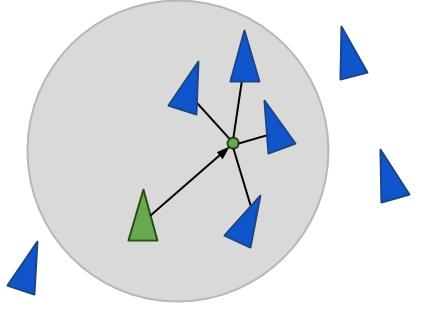
\includegraphics[width=\textwidth]{images/boid_cohesion}
        \caption{Cohesion}
        \label{fig:boid_coh}
    \end{subfigure}
    \hfill
    \begin{subfigure}[b]{0.23\textwidth}
        \centering
        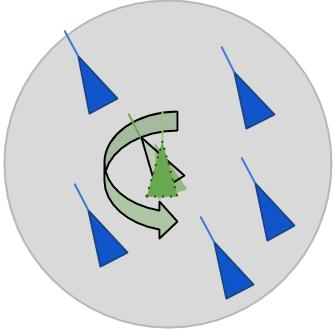
\includegraphics[width=\textwidth]{images/boid_alignment}
        \caption{Alignment}
        \label{fig:boid_ali}
    \end{subfigure}
    \hfill
    \begin{subfigure}[b]{0.3\textwidth}
        \centering
        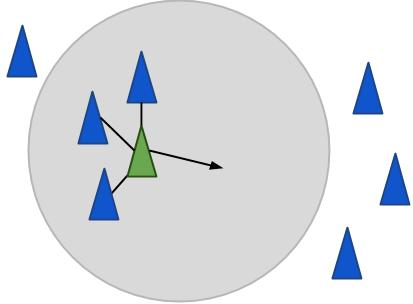
\includegraphics[width=\textwidth]{images/boid_separation}
        \caption{Separation}
        \label{fig:boid_sep}
    \end{subfigure}
    \caption[Boids behavior]{The three behaviors of the Boids}
    \label{fig:boidbehavior}
\end{figure}


%\begin{figure}[H]
%    \centering
%    \subfloat[Separation ]{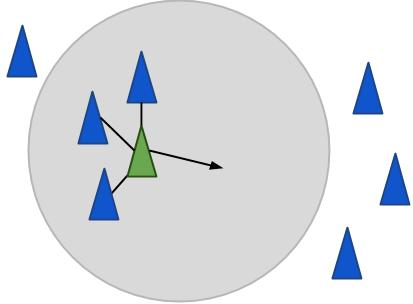
\includegraphics[width=0.3\textwidth]{images/boid_separation.jpg}\label{fig:boid_sep}}
%    \hfill
%    \unskip\ \vrule\ 
%    \subfloat[Alignment ]{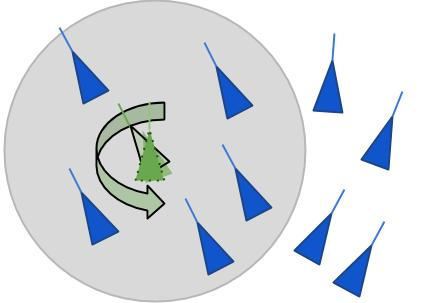
\includegraphics[width=0.3\textwidth]{images/boid_alignment1.jpg}\label{fig:boid_ali}}
%    \hfill
%    \unskip\ \vrule\ 
%    \subfloat[Cohesion ]{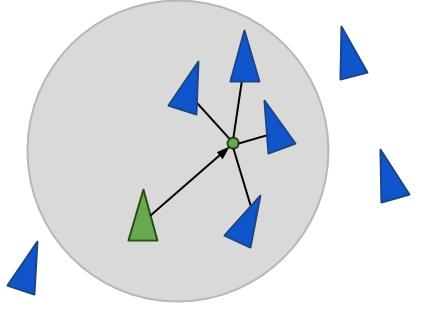
\includegraphics[width=0.3\textwidth]{images/boid_cohesion.jpg}\label{fig:boid_coh}}
%
%            \label{fig:boidbehavior}
%\end{figure}

The three behavior is per individual Boid, which means that each particle/Boid has to calculate where they are going to fly by checking all the other Boids position and rotation and then act accordingly. Which makes the complexity of the algorithm $ O(n^2)$ for every frame. 
Reynolds have tried to make the algorithm less computational expensive by putting the Boids into grids with Spatial Hashing. An example of this could be to put all the Boids that has an $x$-value between 0 and 1 and a $y$-value between 0 and 1 on the lower left grid, and the ones that has an $x$-value between 1 and 2 in the next position etc. Using this grid, each Boids in a cell only needed to take the adjacent grids into consideration when checking their neighborhood. That way they do not need to check the position and rotation of all the other Boids.
\begin{figure}[h!]
    \centering
    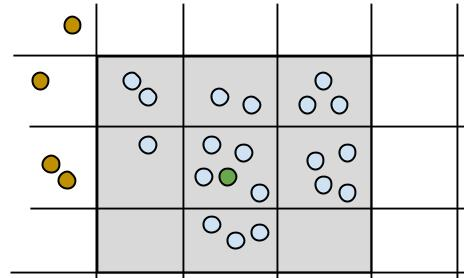
\includegraphics[width=0.8\linewidth]{images/boid_spatialhash}
    \caption{Boids in grids using spatial hash} \label{fig:spatialhash}
\end{figure}
As illustrated in figure \ref{fig:spatialhash}, the green Boid only needs to check the gray Boids that surrounds its own cell, it does not need to check the rotation and position of the orange/brown Boids outside of the gray highlighted area, because they are too far away to be considered a part of its neighborhood.

In another paper \citep{Joselli2009} a different technique were used to optimize 3D swarms, a method using neighborhood grids.

Each Boids to cell ratio would be 1 to 1, that is for every cell, there would be at max 1 Boid. Each Boid would have their respective cell based on their position in space, for instance a Boid with low $x$-value would be on the left of a Boid with higher $x$-value. Boids who are closer to each other in geometric space would be stored closer to each other in the grid. To obtain this, the Boids needs to be sorted. Odd Even sort and Bitonic sort were used as the sorting algorithm. See appendix \ref{app:sorting} for more detail.

Of the two sorting algorithm, Odd Even sort was faster, but not very precise. More than 10\% of the entities were placed in the wrong cell. An Odd Even sort algorithm had to be done for each axis, that is one odd even sort for x, y and z. Each axis were sorted in parallel.
Bitonic Sort on the other hand was slower, but a lot more precise. Less than 1\% of the entities were placed in wrong cell. The reason for placing a Boid in the wrong cell is due to the way the sorting works, it sorts all the entities in one axis first, then a second axis and then the third last axis. For instance sorting on $x$-values first, for the $y$-values, then the $z$-values. When swapping one of the latter axises it might mess up the sorting of one of the other axises.

After the Boids were placed in their corresponding cell, the work could be distributed to the GPU which would calculate where each Boids' new location and rotation would be based on their adjacent neighbor depending on the Moore radius. A Moore radius of 2 would cover the current square, the adjacent squares and their adjacent neighbors as well. The Moore radius is used to determine how many other Boids to consider in its neighborhood. For instance if the Moore radius is 2, the Boids will have a neighborhood as illustrated by the gray color in figure \ref{fig:moore}. Each cell is supposed to contain a Boid.
\begin{figure}[H]
    \centering
    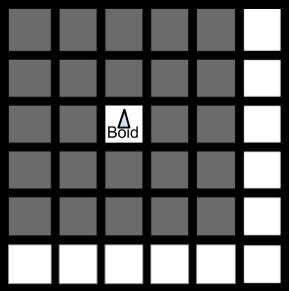
\includegraphics[width=0.3\linewidth]{images/moore}
    \caption[Moore radius illustrated, 2D]{A Moore radius of 2 illustrated by the gray squares}\label{fig:moore}
\end{figure}
In 3D space, extra layers would be added. A Moore radius of 1 would cover all the adjacent grids, which would make the 8 grids that we have in 2D space plus 9 grids above and 9 grids below. That would equal 26 grids, compared to the 8 squares in 2D space. A Moore radius of 2 would cover 74 grids in 3D space (24 + 25 above and 25 below). See figure \ref{fig:3dgrid} for an illustration of the space covered by a Moore radius of 1 in 3D space, this illustration is only an intersection and does not show all the covered grids.
\begin{figure}[H]
    \centering
    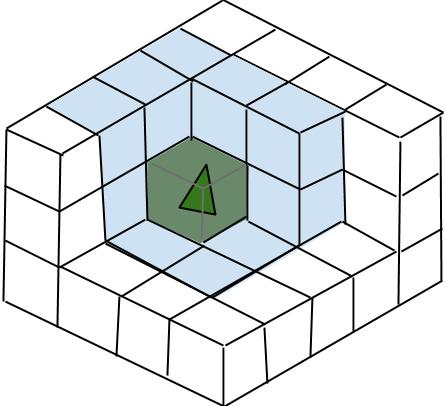
\includegraphics[width=0.5\linewidth]{images/3dgrid}
    \caption[Moore radius illustrated in 3D space]{An intersection of a Moore radius of 1 in 3D space}\label{fig:3dgrid}
\end{figure}

The number of Boids was varied from 1,000 to 1,000,000 and the number of Boid types was varied from 1 to 4. Boids of the same type would try to flock with each other while different types of Boids would try to avoid each other.
They were able to see a speedup compared to the spatial hashing method used by Reynolds, but the Boids were not rendered as a bird or an object, only as a primitive shape. They didn't mention if they tried to add non moving obstacles in their test. Due to the high percentage of Boids being placed in the wrong cell when using odd even sort, a lot of Boids would crash into their neighbor during the test run. However using the neighborhood grid method on GPU, real time simulation of 1 million Boids were possible (6-8 fps).

In the paper "steering behaviors for autonomous character" Reynold discusses steering for autonomous character in games and animation, which is a type of autonomous agent that have some ability to improvise their actions. That means that these agents do not have their actions scripted in advance.
It is possible for the Boids to have more behaviors, called steering behaviors as explained in \citep{Reynolds1999}. The steering behavior decides where the Boids are supposed to steer after their three simple behavior are satisfied.  These steering behavior can be seek, flee, pursuit, evade etc. 

%The \textbf{seek} behavior tells the Boid to seek a goal, it will try to reach the goal/object as fast as possible, and due to the high speed it has when arriving it will fly past the goal. It then turns around to seek the goal again.
%A seek behavior should have an \textbf{arrival} behavior to counteract the fly-by, that means that when nearing the goal, the Boid will slow down so it stops at the goal in the end, instead of flying past it.
%
%A \textbf{flee behavior} is almost the same as the seek, except in the opposite direction. It will try to turn away from the "goal" and fly in the opposite direction or rather fly as far away from the "goal" as possible.
%
%\textbf{Pursuit} is the same as seek, except it applies to moving objects. Pursuit requires prediction of the target's future position. The approach is to predict the future position of the target, reevaluate and readjust it each step. A prediction might be wrong at one time step, but this only applies for that single time step, and a new prediction will be made at the next time step which hopefully will be correct.
%
%An \textbf{offset pursuit} behavior behaves almost the same way as the normal pursuit behavior, except that it will not "crash" into the target but have an offset or $R$. An example of this could be an aircraft flying near the sensors of a base or something similar. 
%
%\textbf{Wander} behavior is a type of random steering, the particle move randomly around, An easy way to implement this behavior is to apply a random steering force each frame, but this leads to twitchy movements, which doesn't look very natural. The proposed method is to have a steering direction which is being displaced each frame with a very small random force.
%That way, if the particle is move forward, it will still keep moving forward the next frame, but it might turn a little bit to the right. Which makes it seem a lot more natural.
%
%\textbf{Path following} behavior enables, as the name suggest, a character to follow a predefined path. However it is not as strict as a train following the rail tracks, the character are allowed to deviate a little bit from the track. The implementation involves a spine with a radius, which makes the track. The path makes a tube in 3D or a thick line in 2D. The goal for the path following behavior is to first reach the tube, then stay inside this tube, thus following the path. Variations of path following are wall following, and containment. Wall following ensures that the character followes the wall, while containment refers to motion restricted inside a region.
%
%\textbf{Leader following} behavior makes one character follow another character. The follower wants to stay near the leader, but also stay out of the way. If there is more than one leader, they also want to avoid bumping into each other. The implementation of leader following behavior relies on the arrival behavior where the goal is a point behind the leader. The follower will slow down when drawing near the point behind the leader and eventually stop before it bumps into the leader. If the entity is in front of the leader, it will fly away and around the leader so it is not in the way.
\begin{description}
\label{boids:behaviors}
\item[The seek]behavior tells the Boid to seek a goal, it will try to reach the goal/object as fast as possible, but due to its high speed it might have when arriving at the goal, it will fly past the goal. It will then turn around to seek its goal again.

A seek behavior should have an \textbf{arrival} behavior to counteract the fly-by, that means that when nearing the goal, the Boid will slow down so it stops at the goal in the end, instead of flying past it.

\item [Flee behavior] is almost the same as the seek, except in the opposite direction. It will try to turn away from the "goal" and fly in the opposite direction and fly as far away from the "goal" as possible.

\item [Pursuit] is the same as seek, except it applies to moving objects. Pursuit requires prediction of the target's future position. The approach is to predict the future position of the target, reevaluate and readjust it each step. A prediction might be wrong at one time step, but this only applies for that single time step, and a new prediction will be made at the next time step which will hopefully be correct.

\item [Offset pursuit] behavior behaves almost the same way as the normal pursuit behavior, except that it will not "crash" into the target, but will have an offset $R$. An example of this could be an aircraft flying near the sensors of a base or something similar. 

\item [Wander] behavior is a type of random steering, where the particle moves randomly around. An easy way to implement this behavior is to apply a random steering force each frame. But this leads to twitchy movements, which does not look very natural. The proposed method is to have a steering direction which is being displaced each frame with a very small random force.
That way, if the particle is move forward, it will still keep moving forward the next frame, but it might turn a little bit to the right. Which makes it seem a lot more natural.

\item [Path following] behavior enables, as the name suggest, a character to follow a predefined path. However it is not as strict as a train following the rail tracks, as the character is allowed to deviate a little bit from the track. The implementation involves a spine with a radius, which makes the track. The path makes a tube in 3D or a thick line in 2D. The goal for the path following behavior is to first reach the tube, then stay inside this tube, thus following the path. Variations of path following are wall following, and containment. Wall following ensures that the character followes the wall, while containment refers to motion restricted inside a region.

\item [Leader following] behavior makes one character follow another character. The follower wants to stay near the leader, but also stay out of the way. If there is more than one leader, they also want to avoid bumping into each other. The implementation of leader following behavior relies on the arrival behavior where the goal is a point behind the leader. The follower will slow down when drawing near the point behind the leader and eventually stop before it bumps into the leader. If the entity is in front of the leader, it will fly away and around the leader so it is not in the way.
\end{description}

\subsection{Not bumping into things}
In the paper \citep{CraigW.Reynolds}, W. Reynolds discusses how to perform obstacle avoidance. That is, obstacles that are placed in the environment which is not a Boid. These obstacles are usually static, non moving obstacles. He starts out with the idea of a force field around the obstacle which he calls the \textit{steer away from surface} approach. The idea is to have every obstacle emit a forcefield around itself which pushed the Boids away. For instance if a Boid is flying toward an obstacle, the obstacle would push the Boid to one side of itself. However this force field method would not work if the Boid flew straight into an obstacle, because the forcefield force would be straight opposite of the direction the Boid is flying thus making the Boid decelerate until it stopped.

The next obstacle avoidance technique Reynold discussed is the curb feeler technique or steer along the wall technique. The idea is to have a feeler that would detect an obstacle before the Boid would crash into it, then turn the Boid away from the obstacle. This can be compared to walking down a dark alleyway where you reach your hand out to feel the walls around you, and navigate through the alleyway just by feeling the wall(s).

The last technique for navigating and avoiding obstacles discussed was image processing. Images could be processed in real time to a gray scale image, where white would signify an obstacle. The algorithm would start with the center of the image, if this was a white pixel it would start to search outwards in a spiral to find either a gray pixel or a black one and then turn the Boid in this direction. This could also be combined with a \textit{Z-buffer image} which gives us a map of the distances to obstacles that lies in front of the Boid, this z-buffer image can be obtained by radar, sonar or similar technology. One interesting way of using the Z-buffer image is to implement a "steer towards the longest clear path". However using this technique without any form of planning or learning might lead the Boid into a local cavity, which might be a dead end.

\subsection{Physic based control system}
In the paper \citep{Spears2004}, a self emergent system was formed using simple attractive and repulsion force for each particle. The idea behind their system was to create an artificial physics framework (AP) that would simulate a physical system. In their paper they had the particles attract other particles that were farther away than distance \textit{r} and a repulsive force is applied if the particles are closer than distance \textit{r}. This leads to the particles always being at distance \textit{r} from each other, which will form a hexagonal lattice. In the hexagonal lattice, each particle will be at a distance $r$ away from each other, but the next neighbor will be $\sqrt{3}r$ away. Therefore each particle only have a vision range of $1.5r$ so they do not affect the particles that are too far away from it. 

In the simulation they spawned all the particles in a cluster, using the two-dimensional Gaussian random variable to initialize the position of the particles. The particles starts with a velocity of 0.0, but their framework does not require so. Due to local forces, the particles will disperse and form local hexagons. To evaluate the quality of the lattice they measured the orientation error of the lattice: they took any particles that were $2r$ apart and formed a line segment, then they took any other particles that were $2r$ apart and formed another line segment. The angle between these to line segments should be measured to be a multiple of $60^{\circ}$. The error would be the absolute value of the difference between the measured angle and the nearest multiple of $60^{\circ}$. The error ranges from $0^{\circ}$ to $30^{\circ}$.

They also checked the size of the particle cluster. For each particle $i$ they counted the number of "close" particles, that is particles that are in the range of $0<r<0.2r$. The minimum cluster size is 1.0 because they count the particle $i$ as well as its neighbors. The cluster count was averaged for all the particles. At the start there was a high cluster count, but it decreased to roughly 2.5 after 6 time steps. 

They also tried out making square patterns, but had to introduce a concept of spin; each particle was either spin "down" or spin "up". Opposite spins would attract each other if the distance was greater than \textit{r}, and repel each other if the distance is less than \textit{r}. If the particles had opposite spin the distance would be $\sqrt{2}r$. This means that all the particles on the vertical space would be alternating between spin up and spin down, the same goes for the particles in the horizontal space. The particles on the diagonal will have the same spins as their diagonal neighbors. Sometimes the formation would have "holes" in it, so instead of static spins, the particles were allowed to change their spin. This would fill in the holes or flaws in the square lattice, according to their theory.

A particle would only change its spin if it had a very close neighbor ($r<1$), and the probability of changing spin was quite small.

\subsection{V like bird formation}
In the paper \citep{Nathan2008}, bird flocking is discussed, they wanted to simulate the V shape that can be observed when birds fly together. They ran a simulation that where each bird individual had 3 simple rules: 
\begin{itemize}
    \item \textbf{Coalescing rule}: \\
        The birds should try to seek the proximity of the nearest bird.
    \item \textbf{Gap-seeking rule}: \\
        If rule 1, the coalescing rule is not applicable anymore the bird should find a position with unobstructed view -  that is, the bird should be able to see in front of it without anything being in the way.
    \item \textbf{Stationing rule}: \\
        Try to stay in place.
\end{itemize}
These rules would make sure that the birds were able to flock and form different shapes. The only thing that was common between the different runs in this paper was that the bird behind would be a little bit behind and slightly left or right of the bird in front (following rule \#2). A lot of different shapes was obtained during the runs, the birds flocked and formed a V-shape, a diagonal line, an inverted V-shape etc.

\subsection{Family bird: A heterogenous simulated flock}
The paper \citep{Demsar2013} by \citeauthor{Demsar2013} says that bird flocks and fish schools seems to be very complex, but the mechanics are very simple as illustrated by Reynold. Only a few simple rules will create flocks that flock together and splits up to avoid obstacles. These flocks are not spectacular or mind blowing compared to the flocks found in nature, due to the rigid motion of each individual. To tackle the artificialness of each individual, Heppner introduced randomness to the motion of the individuals. He defends it by saying that these randomness simulates wind gust, random obstacles and other factors. 
However, the authors of this paper does not agree with this approach because wind gusts will affect the whole flock, not just a random single individual at random. Even with these randomness added, the flock still does not seem lifelike enough compared to their counterpart found in nature. The reason for the lack of breathtaking in these flocking algorithms are that the individuals all have the same characteristics. In nature each individual will have different size, age, form and shape.
 
Usually in flocking algorithms, each individual takes into account where all the other entities are and then act accordingly. In nature, each individual might have limited information about the flock. It might only be able to gain so much from its vision due to other flock members being occluded or not able to hear some of the other individuals due to noise or other factors.

This paper runs a simulation with different types of birds, where social relations are a factor and individuals might be solitary or social. Social individuals are entities who would like to stay close to members of its own social group, for instance a social dove will want to stay with other doves. Solitary individuals on the other hand does not care about staying with its own flock and might drift to another flock. For instance a solitary dove might fly amongst hawks or other types of birds. A flock in this paper are defined as a group where the individuals affect each other in the same group. The simulation they ran varied between all solitary birds to 4 types of different social birds.

\subsection{Particle Swarm Optimization}
Swarms has a lot of potential, not necessary only on robotics but swarms can be used to optimize problem, hence the name \textbf{particle swarm optimization (PSO)} \citep{Eberhart}. PSOs is used to solve problems where optimization are needed. The idea behind PSOs are to have a swarm of particles spawn at random positions in the search space, and then let them fly around searching for solutions. Each particle will know the best solution it have found so far, and the best solution that has been found globally. In some PSO implementations a local best found solution is also known amongst the individual. This local best solution is the best solution amongst a subgroup of individuals and can change for a particle depending on the position of the particle. 

If all of the particles were to be attracted to only the global best found solution so far, they might risk to be stuck in a local maxima without being able to find the other local maximas. To avoid being stuck in a local maxima, each particle is also attracted to the best solution it has found, and maybe to the neighborhood's best found solution as well. This ensure that the particles "jiggles" (introduces enough noise) so that the particle might jump to another local maxima. 

\subsection{Other swarming animals}
This section will look at other flocking animals or insects and how they have been modeled in simulation.
\subsubsection{fishes}
In the paper named "Artificial Fishes: Autonomous Locomotion, Perception, Behavior, and Learning in a Simulated Physical World" \citep{Demetri1994} we are given the explanation on how fishes form schools and how different intentions make the fish behave the way they do. He starts out with explaining how a fish and how the simulator is constructed, the math behind it and how the motor controllers work. For the simulation there is different types of fishes, some of them are predators and some of them are preys. Where predators are larger fishes which tries to eat other smaller preys. Each fish has a 300 degrees, where it can see in front of it and has a blind spot directly behind it. These fish uses the containment behavior mentioned earlier, where they swim freely around in the aquarium, but are not allowed to/not able to leave it.

The range of the vision is also limited and might be occluded by other objects. Each fish has a intention generator, which basically is a flowchart of what the fish needs to do. The prey and predator fish have different intention generators. The predators do not get preyed upon, and thus does not need to look out for other predators, therefore are the intentions of escaping, mating and schooling with other fishes of the same species are disabled. The reason for disabling mating is because there is no need for new predator fishes because they do not die in this simulation. They also do not need to school with other predators because they are not in danger, and do not need the extra survivability.

Whenever a predator sees a prey it will chase the prey if the cost of reaching it is low enough. If it is too high, it will not bother chasing.

Preys on the hand needs the extra survivability, and will try to school with the other fishes if it detects a predator nearby. Each fish will then try to stay a certain distance from the others, which is roughly one body length in distance. Then the fishes will try to adjust its speed and direction so it matches the other members. When this school of fish encounter an obstacle, each individual fish will try to avoid this obstacle. This might lead to the school splitting up and rejoining after they have avoided the obstacle.

A third type of fish introduced here are the pacifists fish. This one differs from the other two type in that the intention of mating is activated while escaping and schooling are deactivated.
The paper describes that there are male and female fishes, and the two behavior which can occur when the fishes start to mate. A behavior named \textit{nuzzling} where the male fish seeks the female and nudges her abdomen until she's ready to spawn, and \textit{spawning ascent} where the female swims repeatedly to the surface while releases gametes. The paper also describes in detail how the fishes select potential partners and how they try to impress each other for mating purposes.

\subsubsection{Ant swarms/colonies}
Ant swarms behaves differently than other types of swarms \citep{Blum2005}, ants do not try to form formations for survival in the same way that birds and fishes do. Ant swarming is mostly about their foraging behavior. That is how they find food for their colony. Each ant's goal is the survival of the colony rather than the survival of each individual. When ants try to find food, they scatter the area by walking in random manner. While exploring the ants leave behind a chemical on the ground. A so called pheromone that the other ants will be able to feel/smell. This pheromone will slowly but surely dissipate. Whenever the explorer ant find a food source, it will evaluate the quality of the food before returning to the anthill. During the return trip, pheromones are reapplied to the path, but the amount is adjusted based on the evaluation of the food. Better food will yield higher pheromone. This method will ensure that the rest of the ants will take the shortest path from the anthill to the food. For the artificial ants, the ant system uses a graph $G = (V,E)$ to model the paths, $V$ are the nodes and $E$ are the edges between the nodes. In the paper \citep{Blum2005}, they use two nodes: $v_s$ which is the starting node or anthill. The node $v_d$ is the food source. There is two ways to reach the food source from the anthill, $e_1$ and $e_2$, which have lengths $l_1$ and $l_2$ where $l_2 > l_1$. A value $\tau_i$ denoted the artificial pheromone, and it indicates the strength of the pheromone. 

An ant will choose a path with the probability $p_i = \frac{\tau_i}{\sum_{ n = 1}^{k}\tau_n}$ where $k$ denotes the number of paths. In the paper, they only have two paths, so the probability of choosing a path is $p_i = \frac{\tau_i}{\tau_1 + \tau_2}, i = 1,2$.
The ant will probably choose $e_1$ if $\tau_1 > \tau_2$ and vice versa.
The ants will return using the same path as the one it took, and reinforce the path with new pheromones using the formula $\tau_i \leftarrow \tau_i + \frac{Q}{l_i}$ where $Q$ is a positive constant. The pheromones that have already been laid out in the path will slowly evaporate, the evaporation formula used is $\tau_i \leftarrow (1-\rho)\cdot\tau_i, i = 1,2$, where $\rho \in (0,1]$. These math formulas will over time make sure that the ants are converging to the short path.

The biggest difference between these artificial ants and real ones are that these move synchronously, while real ants are asynchronous. Real ants leaves pheromones on the ground whenever they move, these artificial ones only leave behind the pheromones on the way back to the anthill. The normal ants' pheromone strength are due to evaporation, while the artificial ones regulates the strength of the pheromones using an evaluation of some quality measure. The ant system can be used for approximate algorithms for combinatorial optimization problem, especially for combinatorial problems which are NP-hard.

\subsection{Robot architectures}
\label{sec:robotArch}
Software architecture is the methodology for structuring the code or algorithm. One software architecture model might work better for one purpose while another architecture works better for a different purpose. 

\begin{figure}[H]
    \centering
    \begin{subfigure}[b]{0.25\textwidth}
        \centering
        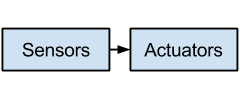
\includegraphics[width=\textwidth]{figs/reactive}
        \caption{reactive control architecture}
        \label{fig:reactive}
    \end{subfigure}
    \hfill
    \begin{subfigure}[b]{0.4\textwidth}
        \centering
        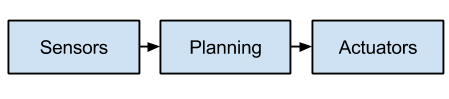
\includegraphics[width=\textwidth]{figs/deliberative}
        \caption{deliberative control architecture}
        \label{fig:deliberative}
    \end{subfigure}
    \hfill
    \begin{subfigure}[b]{0.3\textwidth}
        \centering
        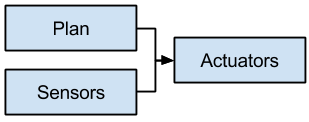
\includegraphics[width=\textwidth]{figs/hybrid}
        \caption{hybrid control architecture}
        \label{fig:hybrid}
    \end{subfigure}
    \caption[Robot architecture]{Robot control architectures}
    \label{fig:robotArchitectures}
\end{figure}

This subsection will briefly explain common architectures found in robotics. In robotics, the architectures needs to decide how to combine reactive control and model-based deliberative planning. Reactive robots relies mostly on their sensor inputs and reacts accordingly. For example a robot equipped with distance sensors that usually drive forward might turn if the front distance sensor detects an obstacle.

Deliberative planning on the other hand also uses the available sensors on the robot, but they do not react immediately like the reactive robots would do. Deliberative planning robots uses the information gathered from the sensor(s) to make a plan of where it should head or what it should do, before executing its action(s).

A mix of both planning and reactive robot architecture which uses reactive techniques at lower level and deliberative planning at the higher levels are called hybrid architectures.

\subsubsection{Brooks subsumption}
\label{sec:brooks}
Brooks subsumption architecture is the most common reactive robot architecture. As explained earlier, a reactive architecture is based on a direct sensor to actuator mapping. That is, whenever a sensor measures anything over a predefined threshold or if the sensor senses anything, the actuator will react immediately. The idea behind the subsumption architecture is to split the behavior of the robot into sub-behaviors into a vertical hierarchy as illustrated in figure \ref{fig:subsumption}. 
\begin{figure}[H]
    \centering
    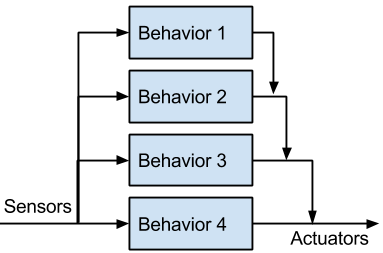
\includegraphics[width=0.5\linewidth]{figs/subsumption}
    \caption[Subsumption architecture]{Subsumption architecture}\label{fig:subsumption}
\end{figure}

As seen in the figure, the sensors input the information it have sensed, and each behavior reacts accordingly. A higher level of behavior will have higher priority than the lower ones. For example, behavior 4 in figure \ref{fig:subsumption} would have priority over behavior 3, and behavior 3 would have priority over behavior 2 etc.


The advantage of the Brooks subsumption architecture is that the robot using it can have different goal depending on the specific situation. For example, if you have a robot that needs to find a specific item in an area. This robot would first wander around aimlessly, and its sensors would be used to avoid crashing into obstacles or other robots. When the robot has located the item it wants, it would use its sensors to move towards that item instead of using it to avoid it, its sensors could be used to align itself with the item to push it towards a different location.

\subsection{Deliberative control architecture}
Deliberative control architecture are based on Sense-Plan-Act principle as seen in figure \ref{fig:deliberative}, the robots uses its sensors to get a full overview of the environment. After it have gained full knowledge of the environment, it will plan solutions then consider them before choosing an action. Deliberative planning robots are usually very dependent on precise sensors to be able to map the environment. It is also assumed that the model of the world the robot will be in is provided. 

\subsubsection{Hybrid control architecture}
\label{sec:hybrid}
Hybrid architecture is a mix of deliberative control architecture and reactive architecture. The idea behind the hybrid control architecture is to work around the limitation and drawbacks of both the reactive and the deliberative control architecture.

\begin{figure}[H]
    \centering
    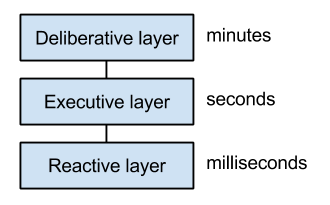
\includegraphics[width=0.5\linewidth]{figs/threelayer}
    \caption[Three layer architecture]{Three layer control architecture}
    \label{fig:threelayer}
\end{figure}

The hybrid control architecture usually have a deliberative layer to plan and model the environment, but the deliberative controls might be slow and not able to act fast enough in certain situations. Each decision might take minutes. The environment that the deliberative layer creates or maps out can be learned from data or gathered through the sensors from the reactive layer.

That is why the reactive layer is added to the control architecture as well. The reactive layer usually have faster reaction time than the deliberate layer, and can help the robot navigate when they need to do an action fast. The reactive layer's decision cycle is often on the order of milliseconds.

To glue together the reactive layer and the deliberative layer, a layer is put in between the lower reactive layer and higher deliberative layer. Namely the executive layer or sequencing layer. The executive layer accepts directive from the deliberative layer and puts them in order for the reactive layer. The executive layer is slower than the reactive layer, it takes seconds to make a decision.

The hybrid architecture explained here is the most common architecture for the hybrid control architecture, which is called the three-layer architecture due to the three layers deliberative, executive and the reactive layer as seen in figure \ref{fig:threelayer}.


\section{Structured Literature Review Protocol}
TODO
%Key words used:
%Swarm
%robotics
%two wheeled differential drive
%Boids
%Birds Flocking
%Fish School
%Ant


%Here you need to include your structured review protocol including search engine, search words, research questions  (for search, not the masters research questions), inclusion createrias and evaluation Criterias. 

\section{Motivation}
\label{sec:motivation}
TODO
%Help CRAB lab further develop the ChIRP robot.



%Your motivation can be either application driven or technique/methodology driven. However in both cases, there will be an element of methodology driven due to the research focus of our group and the nature of a masters project.  
%What other research has been conducted in this area and how is it related to your work? The text should clearly illustrate why your goals and research questions are important to address. This section is thus where your literate review will be presented. It is important when presenting the review that you present an overview of the motivating elements of the work going on in your field and how these relate to your proposal, rather than a list of contributors and what they have done. This means that you need to extract the key important factors for your work and discuss how others have addressed each of these factors and what the advantages/disadvantages are with such approaches. As you mention other authors, you should reference their work. Note that the reference list reflects the literature you have read and have cited. This will only be a subset of the literature that you have read. 

\section{Structured Literature Review Protocol}

%Here you need to include your structured review protocol including search engine, search words, research questions  (for search, not the masters research questions), inclusion createrias and evaluation Criterias. 

\section{Motivation}
\label{sec:no2}

%Your motivation can be either application driven or technique/methodology driven. However in both cases, there will be an element of methodology driven due to the research focus of our group and the nature of a masters project.  
%What other research has been conducted in this area and how is it related to your work? The text should clearly illustrate why your goals and research questions are important to address. This section is thus where your literate review will be presented. It is important when presenting the review that you present an overview of the motivating elements of the work going on in your field and how these relate to your proposal, rather than a list of contributors and what they have done. This means that you need to extract the key important factors for your work and discuss how others have addressed each of these factors and what the advantages/disadvantages are with such approaches. As you mention other authors, you should reference their work. Note that the reference list reflects the literature you have read and have cited. This will only be a subset of the literature that you have read. 
\chapter{Architecture/Model}
\label{cha:architectureAndModel}
This chapter contains the architecture and model of the system, which tools and methods that has been used, how they all connect together to run the experiments and produce the result.
An overview of the system is presented in chapter \ref{sec:overview}. A description of the robot is presented in section \ref{sec:robot}. Section \ref{sec:scenario} contains a description of the different scenarios used in the experiment.

\begin{figure}[h]
\begin{center}
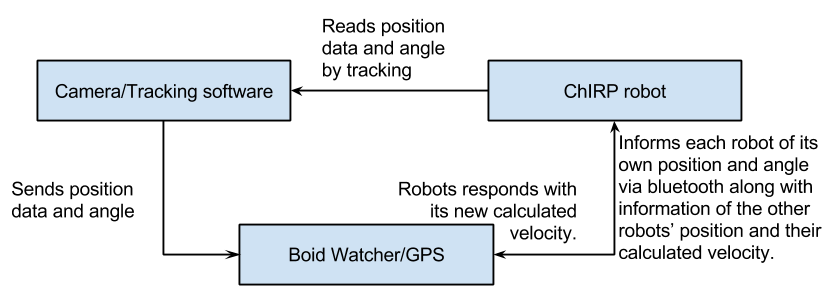
\includegraphics[width=\linewidth]{figs/system_overview}
\end{center}
\caption[System overview]{Overview of the components of the system}
\label{fig:overview}
\end{figure}

\section{System overview}
\label{sec:overview}

The system used in this experiment consists of three primary components as illustrated in figure \ref{fig:overview}: the camera which is used by tracking software, the "Boid-watcher" which is a centralized computer that acts as a GPS and the ChIRP robots.
The camera tracking software tracks each robot's position and its angle, which is sent to the Boid-watcher. The Boid-watcher then forward this information to the robots via the bluetooth serial port.

The Boid watcher does not only work as a GPS but it is also a bridge between the robots, it provides information about the position and velocity of each robot to all the other robots. The robots are not able to connect to the other robots directly, that is why the robots need to pass information to the other robots through the Boids watcher software.

Even if it is possible for one computer to run both the camera tracking and the watcher software, two separate computers were used in this setup. The camera tracking software being run on a stationary desktop computer, and the camera is attached to a pole above a sandbox where the robots roam around. The camera is connected to the stationary desktop. 

In this experiment, the watcher software runs on a laptop with built in bluetooth adapter. The watcher software needs to communicate with all the robots simultaneously and that requires a bit of processing powers.
The desktop computer was not able to run both the camera tracking software and the watcher software at the same time while sending bluetooth data to all four of the robots. When it tried to run both, it was not able to read the data from the camera fast enough and thus the tracking software would crash. The bluetooth connection between the computer and the robots might not always be stable, if the connection were to be unstable at times, a reboot of the robot or/and a reconnection of the bluetooth would usually fix the problem.

The camera tracks the robots using image recognition, it recognizes the robots by the two post it notes that are placed on top of each robot. 
To filter out all the noise from the surrounding and remove the colors that are irrelevant to track, the camera tracking software needs to have a threshold for what it considers to be red and what it considers to be green. This was specified in a configuration file that the camera tracking software loaded whenever it was launched. An example of the configuration file can be seen in the appendix on section \ref{app:opencvcfg}. As seen in the example, each color is defined by six boundaries, a minimum value and a maximum value. If a color seen by the camera is inside this boundary it will be considered as the color it is looking for.\clearpage

\begin{figure}[H]
    \centering
    \begin{subfigure}[b]{0.55\textwidth}
        \centering
        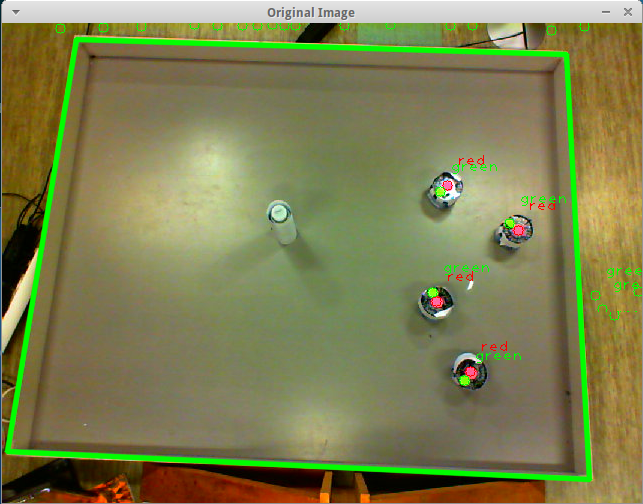
\includegraphics[width=\textwidth]{figs/camOrig}
        \caption{Original image}
        \label{fig:camorig}
    \end{subfigure}
    \hfill
    \begin{subfigure}[b]{0.4\textwidth}
        \centering
        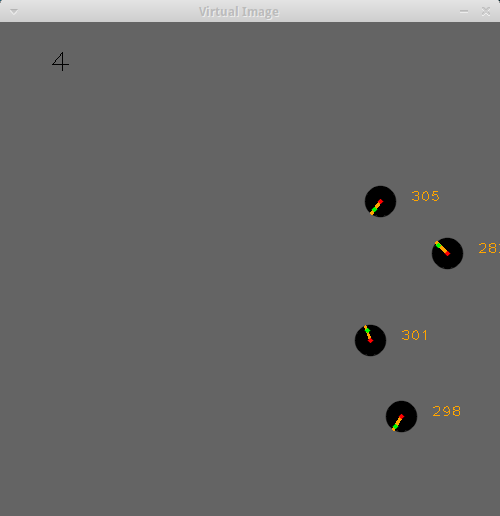
\includegraphics[width=\textwidth]{figs/camVirt}
        \caption{Virtual image}
        \label{fig:camvirt}
    \end{subfigure}
    \caption[Velocity]{Velocity of scenario 1, run 1}
    \label{fig:cam}
\end{figure}

The camera might detect red or green colors that do not belong to the robots, for example when the sun shines into the room, the green part of the floor around the sandbox might be detected as "green" by the camera tracking software. This is not a problem for the camera tracking software, the tracker only tracks inside a predefined box which the user has to specify when starting up the software as seen by the green outline in figure \ref{fig:camorig}. Only the robots inside this predefined area will be tracked and be have a legal position value associated with an angle, any robots found  outside of this green boundary box are not tracked. That is why we need a sandbox to contain the robots so they do not wander off outside the range of the green boundary box where they are not tracked anymore.

Detecting red or green color inside the sandbox that does not belong to the robots' post it notes imposes a bigger problem than detecting these colors outside the box. This might happen if there is a green shaded shadow or a reflection of an object inside the room reflects onto the sandboxes' surface. 
If the software detects green or red color that do not belong to the robot, it is usually not a problem when the green and the red color are far apart from each other, because the camera tracking software does not do anything unless both these colors are paired. If these noise colors do disrupt the movement or angle of the robots, then a recalibration needs to be done to filter out the colors that it should not track.

\section{Robots}
\label{sec:robot}
\begin{figure}[H]
    \centering
    \begin{subfigure}[b]{0.3\textwidth}
        \centering
        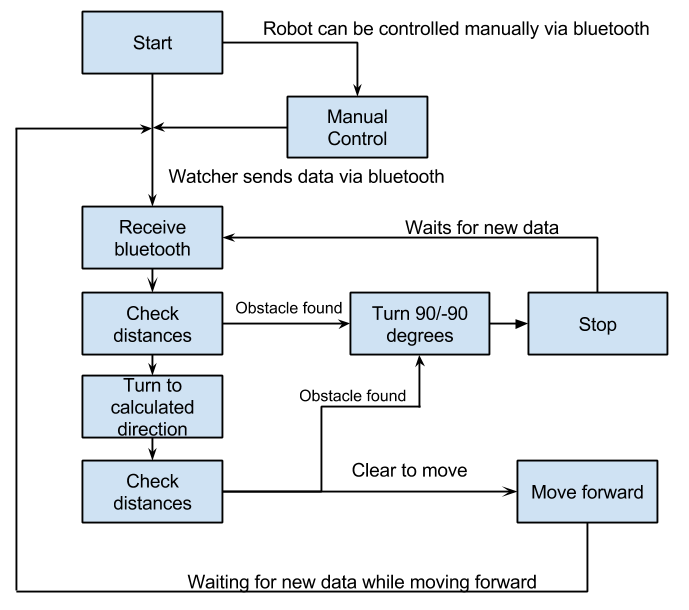
\includegraphics[width=\textwidth]{figs/robotschema.png}
        \caption{$y=x$}
        \label{fig:robot0}
    \end{subfigure}
    \hfill
    \begin{subfigure}[b]{0.3\textwidth}
        \centering
        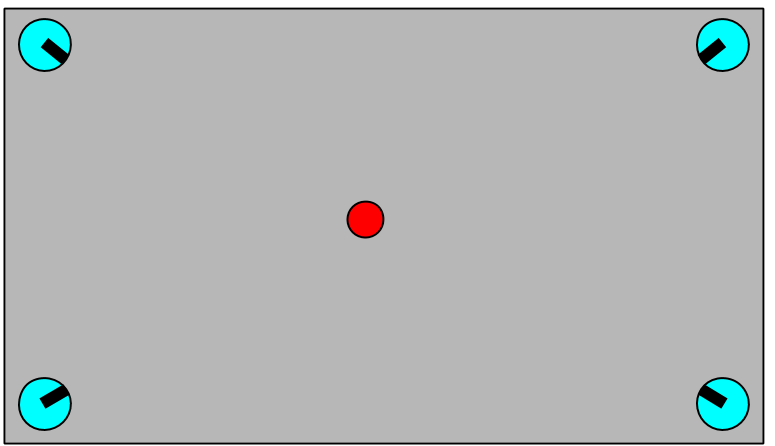
\includegraphics[width=\textwidth]{figs/scenario0.png}
        \caption{$y=3sinx$}
        \label{fig:robot1}
    \end{subfigure}
    \hfill
    \begin{subfigure}[b]{0.3\textwidth}
        \centering
        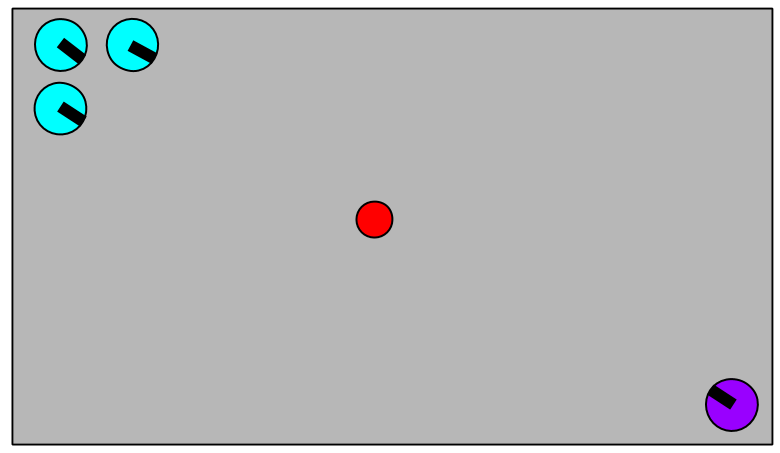
\includegraphics[width=\textwidth]{figs/scenario1.png}
        \caption{$y=5/x$}
        \label{fig:robot2}
    \end{subfigure}
    \caption[ChIRP robot]{ChIRP robot seen from various angles}
    \label{fig:robot}
\end{figure}


The robot swarm consist of four ChIRP robots. The ChIRP robot is a circular shaped robot with differential wheel. A differential wheeled robot is a robot with two separate driven wheels on each side, which it can use move itself. If it wants to change its direction it can vary the relative speed of each wheel or motor. For instance if the right wheel moves faster than the left one, the robot will turn to its left.
The advantage of differential wheel is that an additional steering motor is not required for the robot to move around. Usually a caster or additional wheels are added to balance a differential wheeled robot, but the ChIRP robot does not have anything of the sort. Whenever it is moving, the back or the front of the robot is scraping against the floor depending on if it has a backward or forward momentum. Scraping against the floor does not affect the movement of the ChIRP robot. The robots has a max speed of 13 cm/s, in this experiment the velocity of the robot will not exceed 7.8 cm/s. 

Each robot is equipped with eight infrared LED lights and receivers used for measuring distance. Infrared light are emitted from the LEDs, reflected on a surface and received in the infrared receiver. For the robot to know how far from an obstacle it is, it measures the amount of infrared it receives. The higher the amount, the closer to the object it is. This method of measuring distances works very well for bright or colored surfaces, dark surfaces on the other hand do cause problems because the infrared light is not reflected so well.

The distance sensors are spaced evenly around the robot, where one of the sensors are pointing directly in front of the robot. This sensor can be used to detect whether there is an obstacle directly in front of the robot or not. For this experiment, only the three sensors in front are used. Because the robots only moves forward, so it only needs to determine whether there is an obstacle directly in front of it or not. It does not matter if there is anything behind or next to the robot because it does not move in that direction.

Each of the ChIRP robot is equipped with a bluetooth module, which it uses to communicate with the watcher computer wirelessly. 
The robots are very hollow on top as seen in figure \ref{fig:robot}, and the distance sensors have difficulties sensing other robots due to the hollowness. To counteract the hollowness, a white paper strip was taped around the robots. This makes it easier for the robot to detect the other robots nearby because the paper will reflect the infrared light that the robot uses to determine the distance. To be sure that the robot would be able to detect the obstacles placed in the sandbox, the obstacle would have a white paper wrapped around it to reflect infrared light. The obstacle used for this experiment consist of bottle filled with water. The water inside the bottle is used to make the bottle heavier, so it does not fall over. And the paper around the bottle is there to reflect the infrared light that the robot uses for measuring distances.

The camera tracking software uses image recognition to track the robots. That is why each robot need to have a red and a green post it note on top of it. The red one determines where in the sandbox the robot is located, and the green one is used to determine which way it is pointing and to determine the angle of the robots.

\section{Scenarios}
This section explains the setup of each scenario, where each robot is placed in the sandbox, which way it is rotated and where the obstacle is placed. Each scenario have a purpose to demonstrate, which will be explained more in detail.
For this project experiment, three scenarios have been used to create the results seen in section \ref{sec:results}.
\label{sec:scenario}
\begin{figure}[h]
\begin{center}
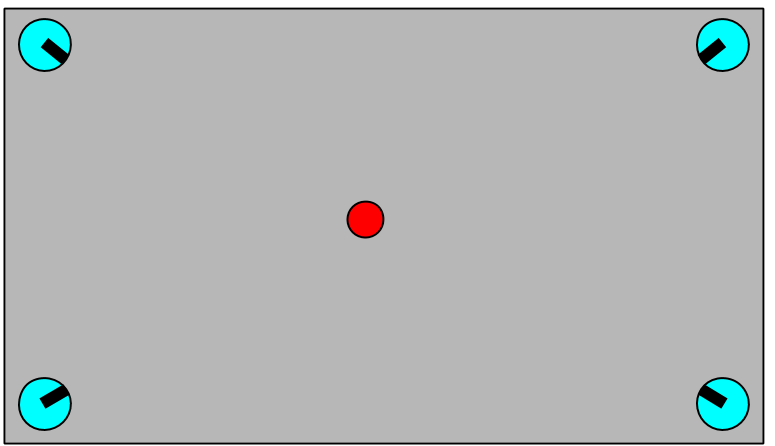
\includegraphics[width=0.8\linewidth]{figs/scenario0}
\end{center}
\caption[scenario 1]{Scenario 1, all the robots are placed in each corner with one obstacle}
\label{fig:scenario1}
\end{figure}

The first scenario is shown in figure \ref{fig:scenario1}, consists of four robots placed on each corner of the sandbox. The reason behind placing each of the robots in each corner of the sandbox is that each robot will be as far from each other as possible. This scenario should demonstrate that the entities are able to flock together, and then stay together as a flock. There is one obstacle placed nearby the middle of the sandbox, the obstacle is placed near the middle to ensure that the robots would encounter it at least once. This scenario would be able to see if the robots actually flocked together like they are supposed to do, and at the same time would be able to avoid the obstacle without bumping or crashing into it. The robots should also move together after they have flocked together.

\begin{figure}[h]
\begin{center}
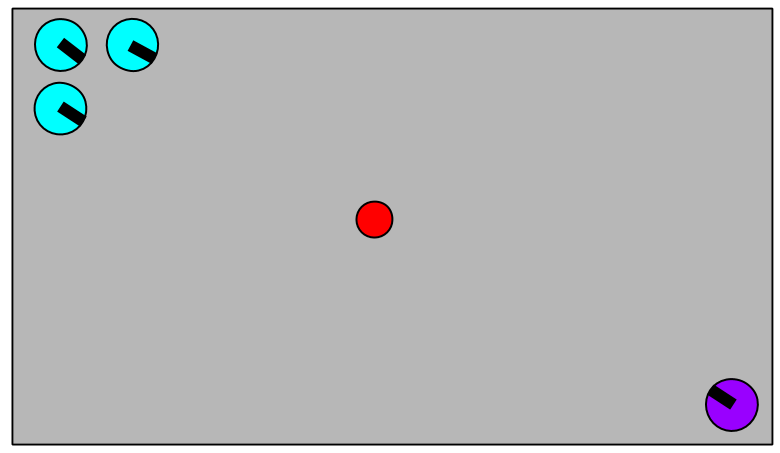
\includegraphics[width=0.8\linewidth]{figs/scenario1}
\end{center}
\caption[scenario 2]{Scenario 2, three robots in one corner, and the last one on the opposite corner}
\label{fig:scenario2}
\end{figure}

The second scenario puts three of entities in one corner, and the last entity is placed on the opposing corner as seen in figure \ref{fig:scenario2}. However the last entity that is placed on the lower right corner by itself will not move, in the case of the physical robot, it will not be turned on. The reason that this entity is a sitting duck placed on the opposite corner of all the other entities is that this robot will act as a goal for the other entities. The obstacle is placed between the lonely robot and the three robots that are clumped up together. The idea behind this setup is that the three robots that start together would try to move to the one that are stationary because they need to flock together. The robot that start by itself does not move because it is not turned on.
The obstacle in the middle will hinder the robots from moving in a straight line to their goal, which forces them to choose a way around it. The robots move around the obstacle when they approach it. As explained in section \ref{sec:robotArch}, the robots will turn either right or left randomly when moving directly towards an obstacle. The robots will probably move around the obstacle on each side of the obstacle, and flock together again on the other side when they have move past the obstacle.

The third scenario is a scenario where the robots are placed randomly around in the sandbox. The two first scenarios were designed for a specific purpose. The purpose of the third scenario is to demonstrate that the Boids behaviors are still intact, even when the robots are placed randomly in the sandbox. The position of the robots, where it should be placed and which way it is pointing was generated randomly by a random number generator. The starting point for this scenario is illustrated in figure \ref{fig:scenario3}. 

This scenario looks a little bit like the first scenario, the robots are laid out in the shape of a square. They are closer to each other than the robots in the first scenario. One of the robots are separated from the other by the obstacle, the robot can not move directly to the other three robots without moving around the obstacle.
\begin{figure}[h!]
\begin{center}
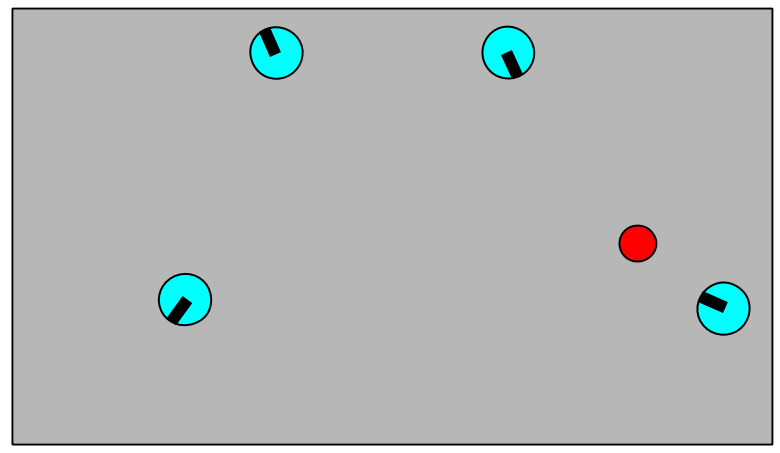
\includegraphics[width=0.8\linewidth]{figs/scenario2}
\end{center}
\caption[scenario 3]{Scenario 3, robots and obstacle randomly placed in the sandbox}
\label{fig:scenario3}
\end{figure}

All the scenarios explained in this thesis uses the same sandbox, which is a sandbox with the size of 151.6 cm wide and 123.9 cm long. The only difference between the scenarios are the placement and rotation of the robots and the placement of the obstacle. Each scenario were run ten times to generate the data seen in section \ref{sec:results}.
In between each run, the robots had to be placed manually back into their starting position before a new run could take place. To keep the data as consistent as possible, everything else would stay as exactly the same.

\section{Robot controller}
This section will go through the controller of the robot, how they work and what steps the robot takes to execute its action.

The robots is implemented using the idea of a hybrid robot control architecture as explained in section \ref{sec:hybrid}. The distances sensors are the reactive layers which will be used to guide the robots away from crashing into other robots, obstacle or walls. The deliberative layer will be the code that processes the data sent from the watcher software on the computer, it calculates where the robot should be heading. The executive layer would be the code running on the robot that decides what the robot is doing, whether that is reading the sensors and avoiding obstacles or towards the planned destination for flocking.

When the robot is turned on and a bluetooth device is paired with its bluetooth module, the robot will stand still and wait. The robot is waiting for a command or data from the watcher software. A human can send commands to manually control the robot if needed, this can be used for leader following as explained in section \ref{boids:behaviors}. 

If the watcher sends data to the robot, it will start to calculate where it should move based on the data it received. 
When the robot have received all the data it needs to be able to calculate its new direction that it should move to. The robot takes into consideration the position of all the other robots, and their velocity. The position of the other robots are used to determine the sum of the cohesion vector and the separation vector. The velocity of the other robots are used to determine which way they are pointing, and this is used to find the alignment vector. 

A fourth behavior was added for this experiment, which is called the "away from wall" behavior. As the name implies, this is a vector that will lead the robot away from the wall of the sandbox if the robot is too near the wall. After calculating each of these vectors, they are multiplied with a weight depending on how much that specific behavior should impact the movement of the robot. For example the separation vector should have higher impact on the movement of the robot because it needs to avoid the other robots when it is too close to one. 

Cohesion vector on the other hand does not need to affect the robot as much, it is mostly there to guide the robot into the flock. Therefore the separation vector is multiplied with a higher number than the other ones.

The equation for how the final vector which decides the direction the robot is going to move is expressed as:
\begin{equation}
\label{eq:vecsum}
\vec{A} = \Sigma_{i=1}^{N_b}(W_i\vec{B_i})
\end{equation}

where:
\\
$\vec{A}$ = the acceleration vector
\\
$B_i$ = the behavior $i$, for example $B_1$ could be cohesion behavior, $B_2$ alignment behavior etc.
\\
$W_i$ = the weight for the behavior $B_i$\\
$N_b$ = the number of behaviors\\

After calculating the acceleration vector, it will add it to its velocity vector, then use the arctangent function to calculate which direction the robot will turn to. The robot calculates the new direction it needs to face by using the following equations:
\begin{equation}
\label{eq:veladdacc}
\vec{V}_{new} = \vec{V}_{old} + \vec{A}
\end{equation}
\begin{equation}
\label{eq:atan2}
R_{goal} = atan2(\vec{V}_y, \vec{V}_x)
\end{equation}
\begin{equation}
\label{eq:angletoturn}
D_{turn} = (R_{goal} - R_{current})* \frac{180}{\pi}
\end{equation}
\begin{equation}
\label{eq:accelreset}
\vec{A} = [0,0]^T
\end{equation}

where:
\\
$\vec{V}_{old}$ = previous velocity of the robot
\\
$\vec{V}_{new}$ = new velocity of the robot, the length of $\vec{V}_{new}$ is capped between -30 and 30 or using mathematic notation: $ |\vec{V}_{new}| \epsilon [-30,30]$.
\\
$R_{goal}$ = the angle the robot will be facing after it has turned around, measured in radians
\\
$R_{current}$ = the angle the robot is currently facing, measured in radians
\\
$D_{turn}$ = the angle the robot needs to turn to face the correct direction, measured in degrees, $D_{turn} \epsilon [-\pi,\pi]$
\\


The robot needs to know how much it is going to move in the x-direction and how much it will move in the y-direction as shown in equation \ref{eq:veladdacc}.
Then by calculating the arctangent of $V_x$ and $V_y$, it finds out which angle it needs to face to be able to move in the direction of $\vec{V_{new}}$. When the robot has calculated which direction it wants to go, it calculates $D_{turn}$ by using the formula in equation \ref{eq:angletoturn}. $D_{turn}$ is the amount of degrees the robot needs to turn to face the right direction. 

The robot will then measure the distances once again, in case it has turned towards an obstacle. If there is no obstacle in front of it, it will move forward and wait for new data from the watcher software. If the robot did find an obstacle in front of it, it will turn 90\textdegree to either the right or the left randomly. The robot will stop after turning and wait for new data from the watcher software. 
\begin{figure}[h!]
\begin{center}
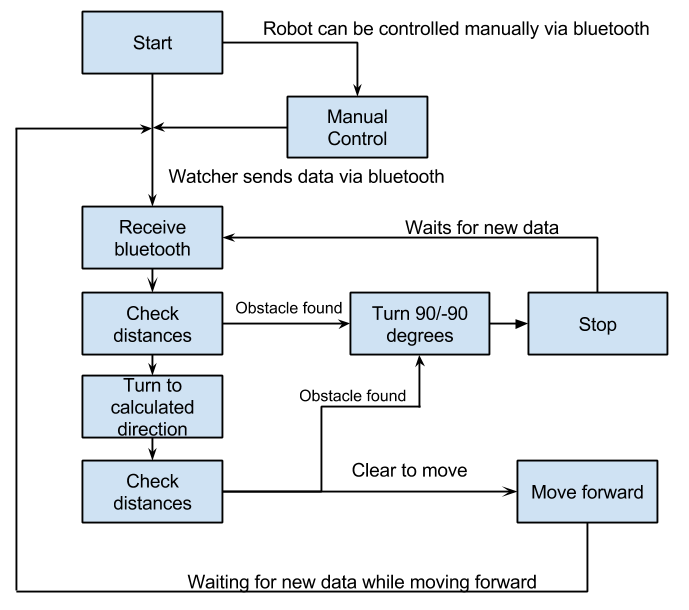
\includegraphics[width=0.8\linewidth]{figs/robotschema}
\end{center}
\caption[Robot flowchart]{Flowchart of the robot's behavior}
\label{fig:robotschema}
\end{figure}
\clearpage

\section{Simulator}
A simulator was created where the Boids was implemented solely in software, and rendered on screen, that is no physical robots were used in the simulator. The reason to use a simulator was to see how the Boids were supposed to behave and have a working example to compare with. A screenshot of the simulator is shown in figure \ref{fig:simulatordistances}.

A typical Boids simulator usually have a wraparound space. If one of the Boids goes outside the window, it will "teleport" to the other side of the window. For example if one of the Boids flies too far to the right and hits the right border, it will loop around and end up on the left side of the screen. That is how the Boids algorithm usually works on a simulator. But physical robots can not loop around the stage like the Boids on the simulator. That is why the simulator used in this project stops the Boids from moving beyond the walls of the window.

The same "away from wall" behavior is also implemented in the simulator, so the Boids do not move into the wall aimlessly.
For each frame, the Boids will update it velocity by calculating a vector for each behavior, and then these vectors are added to the acceleration vector by using the formula found in equation \ref{eq:vecsum}. The acceleration vector is then added to the velocity vector, and the velocity is capped off if the length of the vector exceeds maximum allowed speed. If there is no velocity cap, the Boids' velocity would increase towards infinity. The velocity then decides where the Boids are going to move.
The procedure to calculate the velocity vector of the simulated Boids are the same as the one the robots are using in equation \ref{eq:veladdacc}. 

After calculating the $\vec{V}_{new}$, it needs to cap the max velocity. If the velocity is not capped, the speed of Boids would increase and they would move outside the window. As for the robots, the Boids velocity vector is kept between -30 and 30:  $|\vec{V}_{new}| \epsilon [-30,30]$.
The Boids do not need to calculate which way it needs to turn to move in the direction, because it is able to move in all 360\textdegree\ directions. ing the
The Boids simply moves by adding the velocity vector to their position:
\begin{equation}
\label{eq:posadd}
P_{new} = P_{old} + \vec{V}
\end{equation}

where:\\
$P_{old}$ = old position of the Boid\\
$P_{new}$ = new position of the Boid\\

Before the next time step, the acceleration has to be reset to a null vector for it to work as shown in equation \ref{eq:accelreset}.

The Boids in the simulator does not have any form of rotation, the angle seen on screen are calculated by taking the arctangent of the velocity vector. That is why the Boids in the simulator do not need to rotate; they rotate instantly by changing their velocity.

In the simulator, there is no need for any type of sensors. Each Boid have access to the location of all the obstacles and all the other entities.

Each Boids in the simulator are rendered as a circle, so they are as similar as the real ChIRP bot, however there is some big differences between the real ChIRP robot and the Boids in the simulator. 
%Visually, the Boids are circles on the screen, but all the Boids in the simulator are in fact just a mathematical point with a position. 

\section{Differences between the physical experiment and simulator}
This section will explain the biggest differences between the physical experiment and the simulator. 

The physical robots are trying to mimic the behavior of the Boids created in the simulator. However a physical robot is different than the Boids created in the simulator by nature. As discussed in section \ref{sec:robot}, the robots are a type of differential wheeled robots, which means that it can only move forward or backwards, turn on the spot or move and turn at the same time. It can not move sideways.

The Boids in simulator software did not have any direction, they were able to move freely in all 360\textdegree direction. Which means that if a Boid in simulator were to move in one direction, it could change its momentum and move the other direct without having to stop and turn to that direction. The robot on the other hand would need to turn 180\textdegree before moving forward. The robot is able to reverse its motor to drive backwards, but these Boids robot are not allowed to move backward, and thus have to turn around to move in another direction.

In the simulator, each Boid will know exactly where everything is placed. That is, each Boid knows where all the other Boids are, including itself. It also knows where all the obstacles are. The Boids will have real time access to everything that can be seen on screen. Every Boids will update its perception every frame, that is approximately 60 times every second.

The robots on the other hand, will receive data from the watcher about all the other robots. But due to inaccuracies from the camera and the image processed, the robots only knows vaguely where in the sandbox it is located, and where the others are. The time it takes for a robot to receive new information from the watcher takes roughly one second from the last time it received data from the watcher. If the robots are moving between the time it receives data, it will not know where it is before it receives new data from the watcher software. The camera tracking software are able to see all the robots due to the two post it notes on top, but obstacles found in the sandbox do not contain any color or anything that the camera can track. Obstacles are therefore ignored by the camera tracker software because it does not support tracking of anything other than the robots. That is why the robots needs to use their distance sensors in front to detect the obstacles.

The biggest most visual difference between the physical experiment in the sandbox and the simulated Boids is the size and speed of the entities. The size of the simulator is 1024 px times 1024 px. While the sandbox is 151.6 cm wide and 123.9 cm long, which corresponds to 800x652 px in the watcher software. The Boids on the simulator moves quite fast and can use the extra space to move around, while the robots are confined inside the sandbox. The biggest reason to use 800x652 px for the watcher software is because the behavior neighborhood distances works well for this size.

\begin{figure}[h]
\begin{center}
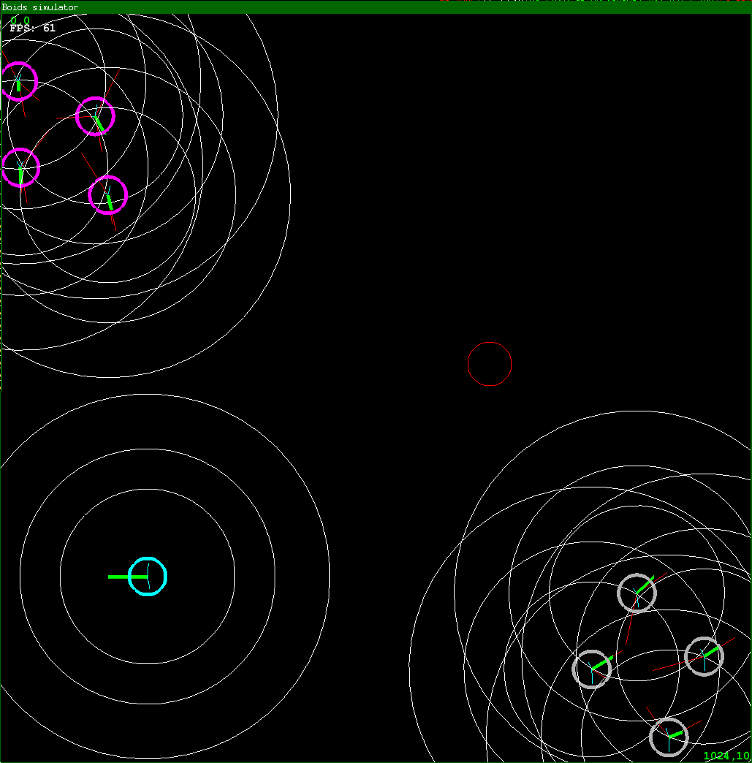
\includegraphics[width=0.8\linewidth]{figs/simulator}
\end{center}
\caption[Simulator distances]{Boids with neighborhood distances visualized}
\label{fig:simulatordistances}
\end{figure}

As it will be explained later in section \ref{sec:experimentalSetup}, the parameters for the simulated Boids and the physical robots are a bit different.
The figure \ref{fig:simulatordistances} shows the approximate distances for each behavior, the inner thick colored ring is the outline of the Boids. The inner thin white ring, illustrates the separation distance, the robot do not try to separate itself from the other robots when they are outside this ring.

The red lines in the figure, is the vectors from each behavior before it is multiplied with the weight. The thickest green line indicates which way the Boids are facing, the longer the line, the faster the Boids are moving.

The second most outer ring indicates the alignment neighborhood, all there is another robot inside this ring, the robot will try to point in the same direction so they move together in the same direction.

The outer circle is the cohesion distance, the Boids outside of this box will not attract each other.


In the figure \ref{fig:simulatordistances}, three types of Boids exist, each one have their own color. Boids will flock together and align themselves only if they have the same color, that is the light gray Boids will flock together with the other light gray Boids. The magenta Boids will only flock together with the other magenta Boids.
When running the simulation for the experiment, all four of the Boids were the same color, therefore just one flock of Boids would emerge instead of forming multiple flocks. The current implementation of the Boids algorithm on the robots do not support multiple groups of Boids. There is no point in implementing this functionality when there are only four robots running at the same time, because it will be very hard to distinguish the difference between a family group flock or if there is just a robot astray from the flock.

\begin{figure}[h]
\begin{center}
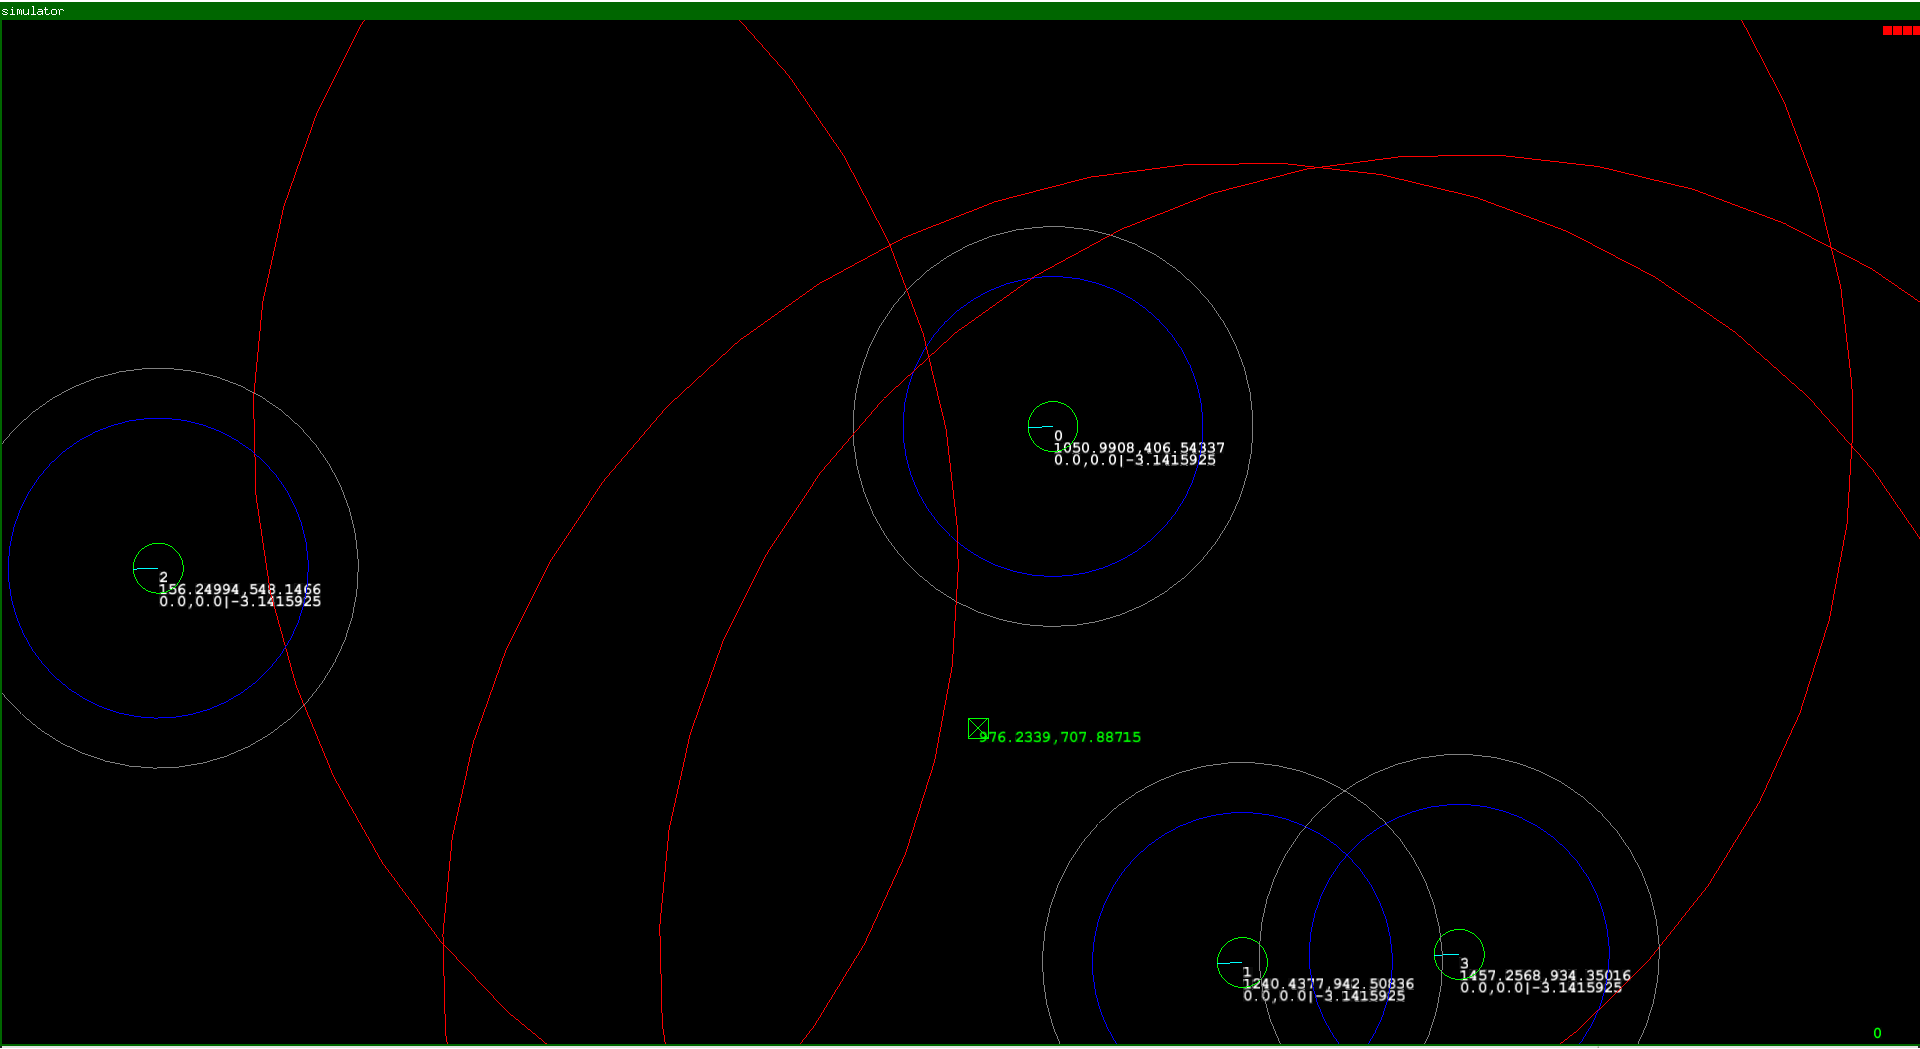
\includegraphics[width=1.1\linewidth]{figs/wathcer}
\end{center}
\caption[Watcher software]{Watcher software with neighborhood distances visualized}
\label{fig:watcher}
\end{figure}

Figure \ref{fig:watcher} illustrates the distances that the robots uses. The exact numbers can be found in section \ref{sec:experimentalSetup}. The distances have been colored for convenience, because it is hard to see which ring represents which behavior. As in the simulator, the most inner ring, which is green in this figure represents the outline of the robot. The figure shown is not the same size as the watcher software that is used to run the experiments, the resolution of the watcher software on the figure has a resolution of 1024x1920 px which is a lot bigger than the resolution on the watcher software used in the experiment. This is to make it easier to see and distinguish the distances.

The next ring, which is illustrated with a blue color, represents the separation distance. And the gray ring shows the alignment neighborhood distance. These two distances are the same in the simulator and on the robot.

The biggest red ring is the one that is the most different from the simulator's. The robots might get stuck in a corner, or drive around in circles.
The reason the cohesion distance is so large is mainly to force the robots to flock together even when their are far apart. The distance almost covers the whole sandbox, that way the robots will try to flock from almost anywhere in the sandbox.

Information about each robot is also provided by the numbers next to each robot.
The first row show us the ID of the robot, and the serial port that belongs to that robot if there is a bluetooth connection and it is assigned.
Second row shows us the position of the robot, while the third one shows velocity and the angle of the robot.

The upper right red squares indicates whether the bluetooth connection is still functional or if the bluetooth have timed out. The squares in the figure are all red, because this is just a debug run where there is no bluetooth connection.


\chapter{Experiments and Results}
\label{cha:ResearchAndResults}

{\it In this chapter, the results from the experiments will be presented and discussed. Section \ref{sec:results} contains the actual results created by running each scenario. The setup of the experiment is explained in section \ref{sec:experimentalSetup}, it explains the setup and which parameters have been used to run the experiments.
Section \ref{sec:discussion} will discuss the results seen in section \ref{sec:results}, and a discussion on the differences between the results from the simulator and the physical robots.}

\section{Experimental Plan}
\label{sec:experimentalPlan}
To be able to test whether the robots are behaving like the Boids, and graphs are plotted to compare the difference between the Boids and the robots. 
Three scenarios or three different starting position will be used as explained in section \ref{sec:experimentalSetup}.
For the physical experiment with the robots, each scenario will be ran ten times to generate the graphs for the results, while only five runs will be used for plotting the behaviors of the simulated Boids. 
If the simulator runs a scenario twice, that is two different simulations with the same parameters and starting position of the Boids are ran, the Boids in the two simulations would start by moving in the exact same way. That is why only five runs were used to generate the results.
The robots did not behave as deterministic as the Boids, there are many factors that can affect the movement of the robots. For example if there are other people moving around in the room where the experiment where the light setting could be affected enough so the camera would not be able to recognize the two post it notes on top of the robot, thus the camera tracking software would not be able to recognize the robots.
Therefore ten runs were used to generate the results when running the experiment on the physical robots. 
All of the results for each scenario was then added together and divided by the number of runs used on that experiment to make the plot show the average of all the runs.
Namely the distance between the entities, angle difference between the entities and the velocity are the features the software will use when creating the results.
The distance between the entities is used to determine if the entities are flocked or not, the lower the distance, the closer they are to one another.
The angle difference are used to check if they are looking in the same direction, if all of the entities are looking in the same direction, the angle difference would be 0.
%Using only the angle difference and the distance between each entity is not sufficient to determine whether the Boids behavior is working or not, because the robots might flock together, face the same direction then stand still there. That is why the velocity are plotted as well.
%TODO, write about how the experiments were ran.

%from template: Trying and failing is a major part of research. However, to have a chance of success you need a plan driving the experimental research, just as you need a plan for your literature search. Further, plans are made to be revised and this revision ensures that any further decisions made are in line with the work already completed. The plan should include what experiments or series of experiments are planned and what question the individual or set of experiments aim to answer. Such questions should be connected to your research questions so that in the evaluation of your results you can discuss the results wrt to the research questions.  

\section{Experimental Setup}
\label{sec:experimentalSetup}
%In this section, the setup for the experiment will be explained, and which parameters have been used to run the experiments. 
This section explains the setup of each scenario, where each robot is placed in the sandbox, which way it is rotated and where the obstacle is placed. Each scenario have a purpose to demonstrate, which will be explained more in detail.
In this experiment, four robots and one obstacle is used inside a sandbox. Each robots needs to have an extra layer on top of them so the red and green post it note does not fall off as seen in figure \ref{fig:robot0}. The robots moves inside a sandbox, which is watched by a web camera from above.

For this project experiment, three scenarios have been used to create the results seen in section \ref{sec:results}.
\label{sec:scenario}
\begin{figure}[h]
\begin{center}
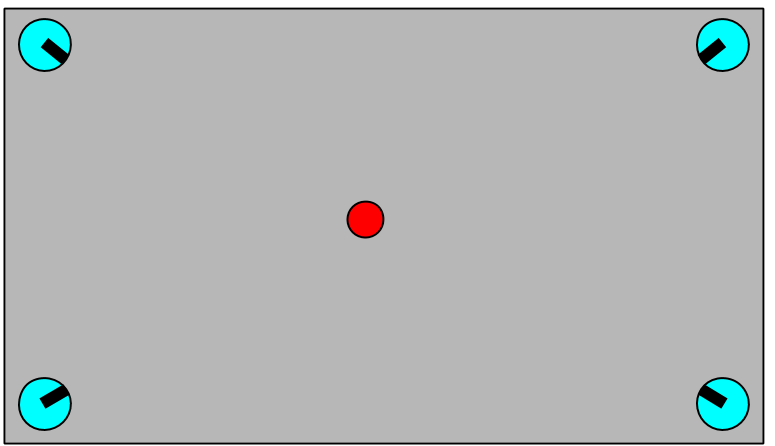
\includegraphics[width=0.8\linewidth]{figs/scenario0}
\end{center}
\caption[scenario 1]{Scenario 1, all the robots are placed in each corner with one obstacle}
\label{fig:scenario1}
\end{figure}

The first scenario is shown in figure \ref{fig:scenario1}, consists of four robots placed on each corner of the sandbox. The reason behind placing each of the robots in each corner of the sandbox is that each robot will be as far from each other as possible. This scenario should demonstrate that the entities are able to flock together, and then stay together as a flock. There is one obstacle placed nearby the middle of the sandbox, the obstacle is placed near the middle to ensure that the robots would encounter it at least once. This scenario would be able to see if the robots actually flocked together like they are supposed to do, and at the same time would be able to avoid the obstacle without bumping or crashing into it. The robots should also move together after they have flocked together.

\begin{figure}[h]
\begin{center}
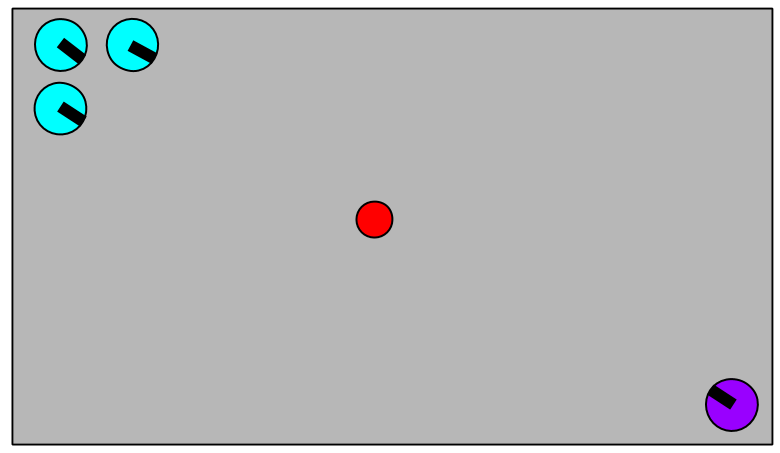
\includegraphics[width=0.8\linewidth]{figs/scenario1}
\end{center}
\caption[scenario 2]{Scenario 2, three robots in one corner, and the last one on the opposite corner}
\label{fig:scenario2}
\end{figure}

The second scenario puts three of entities in one corner, and the last entity is placed on the opposing corner as seen in figure \ref{fig:scenario2}. However the last entity that is placed on the lower right corner by itself will not move, in the case of the physical robot, it will not be turned on. The reason that this entity is a sitting duck placed on the opposite corner of all the other entities is that this robot will act as a goal for the other entities. The obstacle is placed between the lonely robot and the three robots that are clumped up together. The idea behind this setup is that the three robots that start together would try to move to the one that are stationary because they need to flock together. The robot that start by itself does not move because it is not turned on.
The obstacle in the middle will hinder the robots from moving in a straight line to their goal, which forces them to choose a way around it. The robots move around the obstacle when they approach it. As explained in section \ref{sec:robotArch}, the robots will turn either right or left randomly when moving directly towards an obstacle. The robots will probably move around the obstacle on each side of the obstacle, and flock together again on the other side when they have move past the obstacle.

The third scenario is a scenario where the robots are placed randomly around in the sandbox. The two first scenarios were designed for a specific purpose. The purpose of the third scenario is to demonstrate that the Boids behaviors are still intact, even when the robots are placed randomly in the sandbox. The position of the robots, where it should be placed and which way it is pointing was generated randomly by a random number generator. The starting point for this scenario is illustrated in figure \ref{fig:scenario3}. 

This scenario looks a little bit like the first scenario, the robots are laid out in the shape of a square. They are closer to each other than the robots in the first scenario. One of the robots are separated from the other by starting behind the obstacle, the robot can not move directly to the other three robots without first moving around the obstacle.
\begin{figure}[h!]
\begin{center}
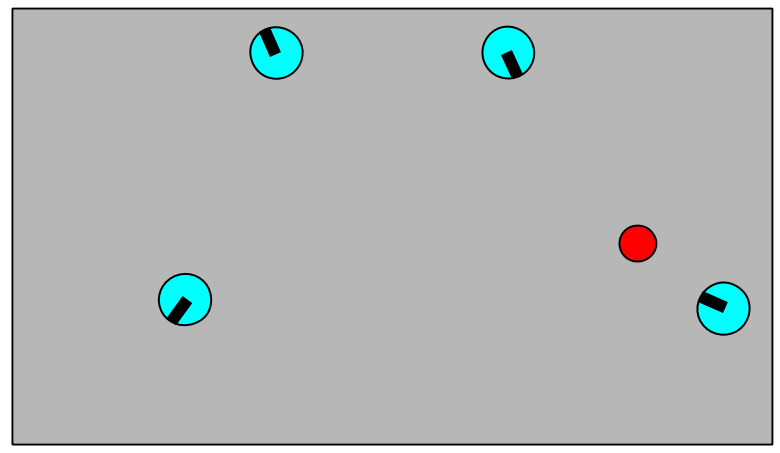
\includegraphics[width=0.8\linewidth]{figs/scenario2}
\end{center}
\caption[scenario 3]{Scenario 3, robots and obstacle randomly placed in the sandbox}
\label{fig:scenario3}
\end{figure}

All the scenarios explained in this thesis uses the same sandbox, which is a sandbox with the size of 151.6 cm wide and 123.9 cm long. The only difference between the scenarios are the placement and rotation of the robots and the placement of the obstacle. Each scenario were run ten times to generate the data seen in section \ref{sec:results}.
In between each run, the robots had to be placed manually back into their starting position before a new run could take place. To keep the data as consistent as possible, everything else would stay as exactly the same.
For the experiments on the simulator, only five runs will be used. Boids have the same starting position and the same direction each time, each run is therefore not very different from the other ones. 

The camera used in this experiment is a web camera. To be able to get a clear stable video feed images from the web camera, the settings for the camera had to be manually set up.
The most important setting is to disable auto focus. Auto focus makes the images blurry, and the camera tracking software will not be able to detect red and green colors which defines the robots. 50 Hz power line frequency was used instead of 60 Hz to eliminate flickering on the camera feed. The other settings are not that important, as long as the web camera is able to provide a decent looking image that the camera tracker software is able to recognize. 

%The experimental setup should include all data - parameters etc, that would allow a person to repeat your experiments. 


\section{Results}
\label{sec:results}

The Boids algorithm are supposed to keep the robots flocked together and preferably they should face the same direction as well. The watcher knows where each robot is, and it knows which direction each robot is facing. The watcher measures the distance between each robot and the angle difference between the robots every five frame or twelve times each second, it then calculates the mean and standard deviation of the distances and angles and saves it to a file. The mean and standard deviation of the velocity is recorded as well, in the simulator the velocity is measured directly by getting the velocity vector on each object, for the physical robot, the change in position is measured instead.

To keep the data as consistent between each run the watcher stops all the robots and saves the data file exactly three minutes or 180,000 milliseconds after the robots have started to move.
The distance measured are in pixels. The measurement of the sandbox is 151.6 cm wide and 123.9 cm long. The watcher software creates a window that has a resolution 800x652 pixels, which means that 1 cm is approximately 5.3 pixels on the screen. The measured angles are shown in radians.

In the upcoming figures, the results from the various runs will be shown. On the x-axis the time will be shown, and the y-axis displays various types of data is presented depending on the figure. The time shown on the x-axis displays the iteration, and not seconds. One iteration is five frames, the software runs with a 60 frames per second. Which means that twelve iterations on the x-axis corresponds to one second. The velocity is measured every iteration, the velocity graph is mostly used as an indication to whether the robots are moving or not. The velocity graphs can be used as an indication whether the robots are moving fast or slower, but it can not be used to reliably tell the velocity of the robots. The velocity graph for the simulated Boids are more precise.
The number shown on the y-axis shows the average length of the velocity vector for each Boid.

The upcoming figures will show graphs of various types, two similar ones will be displayed for each scenario. One is the results from ten runs on the physical experiment with the robots, and the other one is the results from the experiments ran in simulation. In section \ref{sec:discussion} a discussion of the results will be presented, it will contain an explanation as to why some of the graphs might be different.

\subsection{Results from scenario 1}
\label{sec:res1}
\begin{figure}[h]
\begin{center}
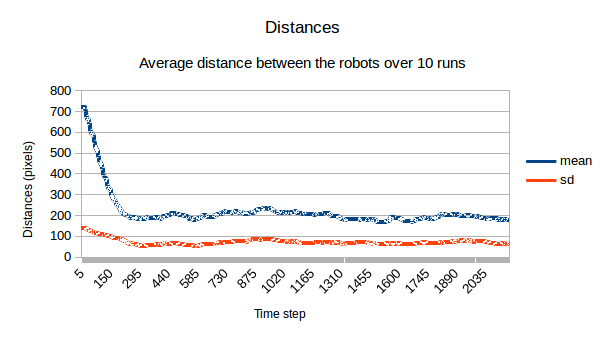
\includegraphics[width=0.8\linewidth]{figs/runs/1pdist}
\end{center}
\caption[1. Distances, robots]{Results from 10 runs averaged on scenario 1, robots}
\label{fig:res1pdist}
\end{figure}
\begin{figure}[h]
\begin{center}
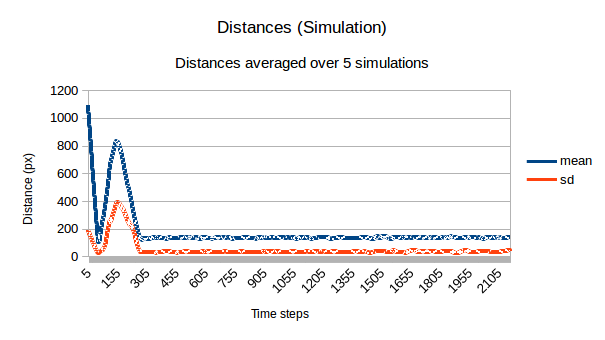
\includegraphics[width=0.8\linewidth]{figs/runs/1sdist}
\end{center}
\caption[1. Distances, simulation]{Results from 5 runs averaged on scenario 1, simulator}
\label{fig:res1sdist}
\end{figure}
%See figure \ref{fig:scene1peakillustrated}. %TODO
%\begin{figure}[h]
%\begin{center}
%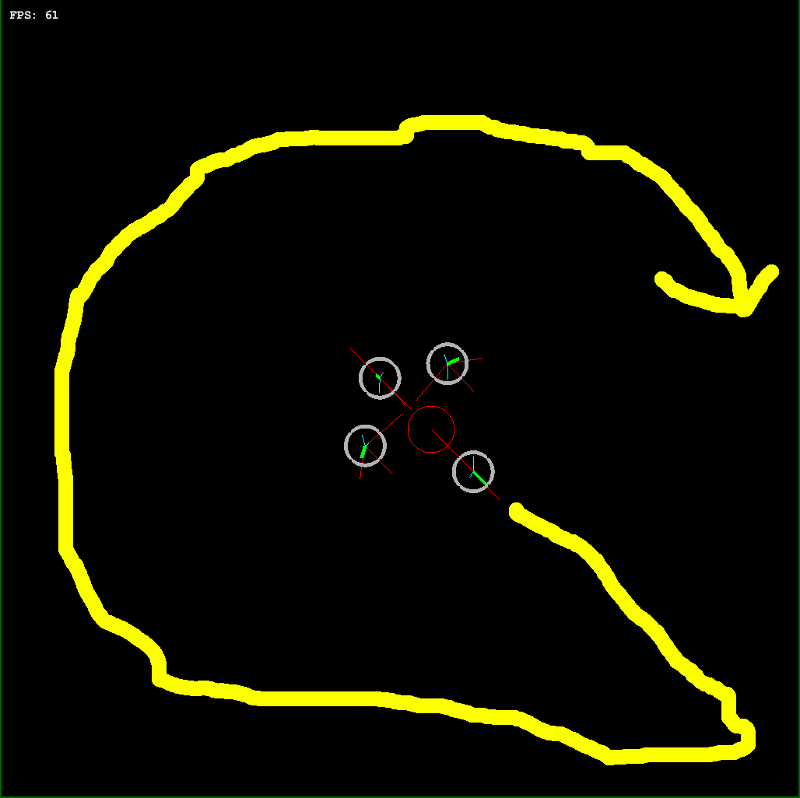
\includegraphics[width=0.8\linewidth]{figs/scene1_pushedaway2}
%\end{center}
%\caption[3. Velocity, robots]{Results from 10 runs averaged on scenario 3, simulator}
%\label{fig:scene1peakillustrated}
%\end{figure}
The first scenario was designed to check if the robots were able to flock together, the robots were placed on each of its corner, as far from each other as possible.
From the figure \ref{fig:res1pdist} we can see that the robots are flocking together quite fast, they start out on each corner of the sandbox then move towards the center of the sandbox, this is shown in the graph by the first drop from 700 px to around 200 px. This corresponds to roughly 132 cm to 37 cm. The time it takes for the graph to drop from 700 px to 200 px is around 300 iterations, which equals 25 seconds.
The simulated Boids behave differently in the same scenario, as seen from figure \ref{fig:res1sdist}, between time step 40 and 305, the graph shows a local maxima. Because all of the Boids are moving towards the middle due to the velocity they have at the start, the distance between them will decrease. But one of the Boids is moving directly toward the obstacle and facing it directly, when it comes too close, it will be "pushed" directly in the opposite direction. The Boid that is being "pushed" in the opposite direction by the obstacle is too far away from the other Boids for the cohesion behavior to be active, and therefore moves away from the rest of the flock. This is the reason there is a peak in the graph.

\begin{figure}[h]
\begin{center}
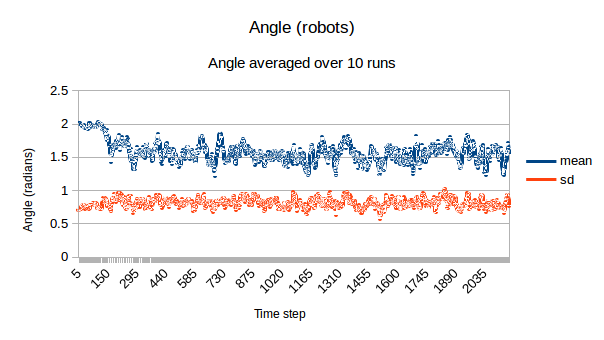
\includegraphics[width=0.8\linewidth]{figs/runs/1pangle}
\end{center}
\caption[1. Angle, robots]{Results from 10 runs averaged on scenario 1, robots}
\label{fig:res1pang}
\end{figure}
\begin{figure}[h]
\begin{center}
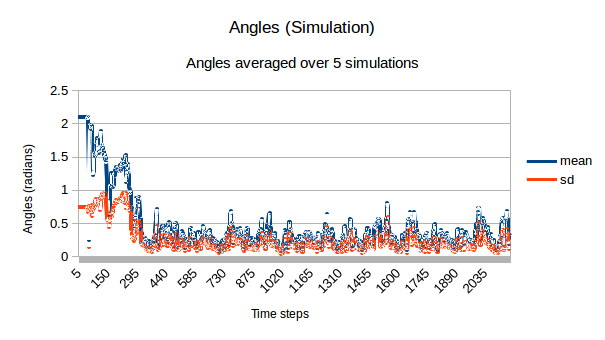
\includegraphics[width=0.8\linewidth]{figs/runs/1sangle}
\end{center}
\caption[1. Angle, Simulation]{Results from 5 runs averaged on scenario 1, simulator}
\label{fig:res1sang}
\end{figure}

In this scenario, the difference between the angles of the robots starts at 2 radians. This is when all of the robots are facing towards the center of the sandbox. After the robots have moved towards the center, they will start to turn around and the difference between the robots decreases. However, the robots are not able to face the same direction entirely, the lowest difference is still above 1.2 radians, which is approximately 68 degrees. 
The simulated Boids' angle also starts at approximately 2 radians, then slowly decreasing to 0.3 radians. When the graph has flattened out at 0.3 radians, it seems like all the Boids are facing in the same direction.


\begin{figure}[h]
\begin{center}
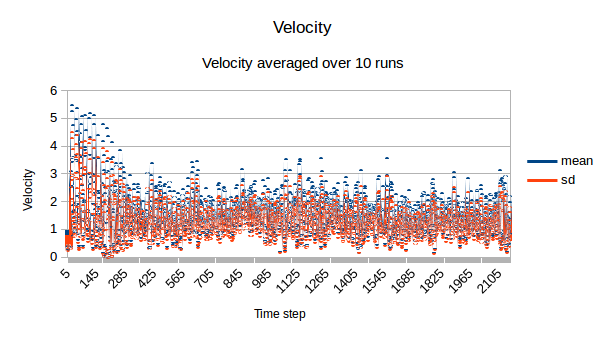
\includegraphics[width=0.8\linewidth]{figs/runs/1pvel}
\end{center}
\caption[1. Velocity, robots]{Results from 10 runs averaged on scenario 1, robots}
\label{fig:res1pvel}
\end{figure}
\begin{figure}[h]
\begin{center}
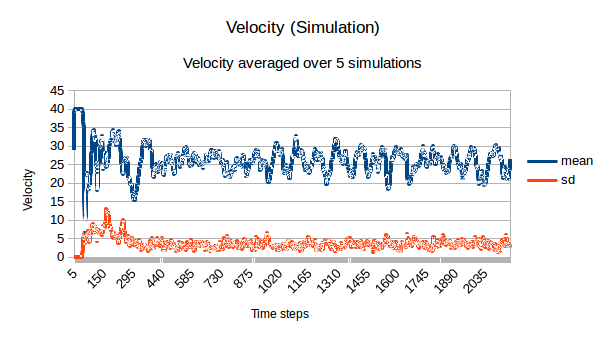
\includegraphics[width=0.8\linewidth]{figs/runs/1svel}
\end{center}
\caption[1. Velocity, simulation]{Results from 5 runs averaged on scenario 1, simulator}
\label{fig:res1svel}
\end{figure}
Both the robots and the Boids have high velocity at the start when they are moving towards the center. When the Boids reaches the center of the simulated space, they will need to adjust their velocity to change direction, and when all four Boids move together as a flock unit, they need to adjust their flight direction all the time. 
The velocity graph for the robot in this scenario has the same general outline as the simulated Boids; the graph shows a high velocity at the start, then drops down before stabilizing at a given range. The robots' velocity jiggles a lot, ranging 0.1 to 3.6, there might be various reasons for this result will be discussed more in depth in section \ref{sec:discussion}.
\clearpage
\subsection{Results from scenario 2}
\label{sec:res2}
\begin{figure}[h]
\begin{center}
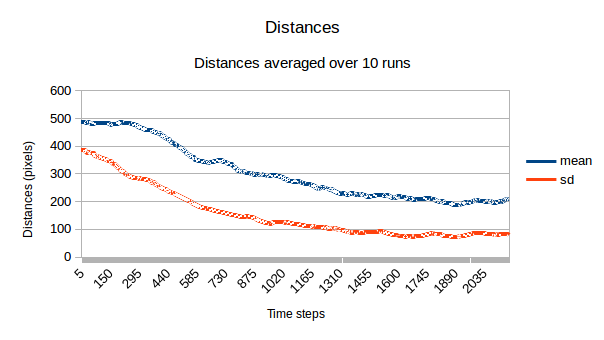
\includegraphics[width=0.8\linewidth]{figs/runs/2pdist}
\end{center}
\caption[2. Distances, robots]{Results from 10 runs averaged on scenario 2, robots}
\label{fig:res2pdist}
\end{figure}
\begin{figure}[h]
\begin{center}
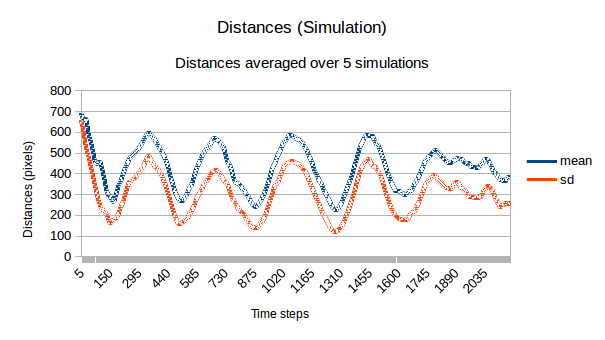
\includegraphics[width=0.8\linewidth]{figs/runs/2sdist}
\end{center}
\caption[2. Distances, simulation]{Results from 5 runs averaged on scenario 2, simulator}
\label{fig:res2sdist}
\end{figure}
Earlier demonstrations of Boids have shown us that when a flock of Boids are moving towards an obstacle, the Boids would split up to sub-groups, fly around the obstacle before merging together on the other side. This scenario is designed to check if this behavior is still intact.

In the second scenario, it takes a bit longer for the distance to drop to 200 px, around 1310 time steps, which is approximately 110 seconds.
Three of the robots are already in a flock while the fourth one is astray from the flock on the opposite side of the sandbox. The three robots that have already flocked together will try to stay together, they do not want to move all the way to the other side to flock with one single robot. If all of the robots were moving, the single robot would move towards the three robots and they all would flock together faster.

When running scenario 2 on the simulator, the Boids move towards the obstacle and around it. When they are near enough to the non-moving Boids, the cohesion behavior will activate and the Boids will try to flock, but all the other behaviors are trying to push the three moving Boids away from the non-moving Boid. After being pushed away, they will keep moving in the same direction and move all the way around the screen. This movement around the screen creates the oscillated graph seen in figure \ref{fig:res2sdist}.

\begin{figure}[h]
\begin{center}
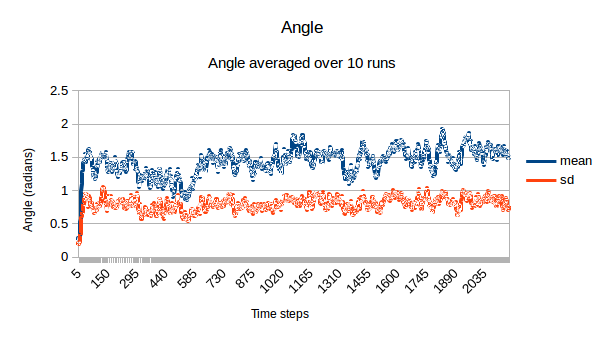
\includegraphics[width=0.8\linewidth]{figs/runs/2pangle}
\end{center}
\caption[2. Angle, robots]{Results from 10 runs averaged on scenario 2, robots}
\label{fig:res2pang}
\end{figure}
\begin{figure}[h]
\begin{center}
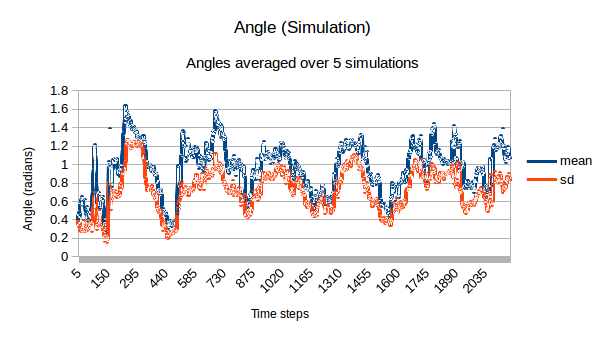
\includegraphics[width=0.8\linewidth]{figs/runs/2sangle}
\end{center}
\caption[2. Angles, robots]{Results from 5 runs averaged on scenario 2, simulator}
\label{fig:res2sang}
\end{figure}
In the second scenario, one of the entity is stationary, and thus its angle does not change, but its angle is still accounted for when the graphs were created. The angles shown in the graphs for the second scenario starts in the lower end, then increases.
Three of the entities starts by facing the same direction, while the last stationary one faces in the opposite direction. That is, all off them faces toward the center as seen in figure \ref{fig:scenario2}.
When starting the runs for the second scenario, the robots started to turn around immediately, thus increasing the difference-angle shown in the graph. One of the robot starts in the upper left corner, it is covered by the two other robot, having no way to move out of this corner without colliding into the other robots, its only option is to turn around on the spot.

The three moving Boids starts off by moving towards the center of the screen, they then move around the obstacle. After reaching the stationary Boid, they are pushed away, which forces them to turn away from the stationary Boid. The Boids angles follows a wave pattern, much like the distances.

\begin{figure}[h]
\begin{center}
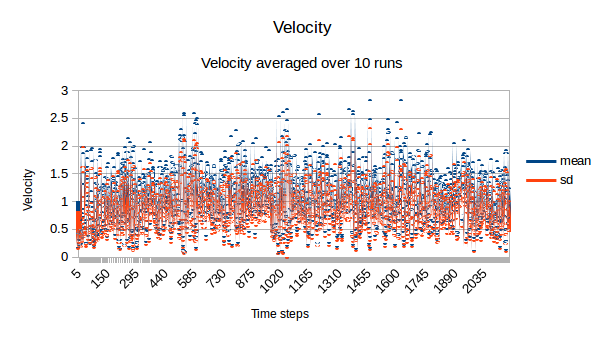
\includegraphics[width=0.8\linewidth]{figs/runs/2pvel}
\end{center}
\caption[2. Velocity, robots]{Results from 10 runs averaged on scenario 2, robots}
\label{fig:res2pvel}
\end{figure}
\begin{figure}[h]
\begin{center}
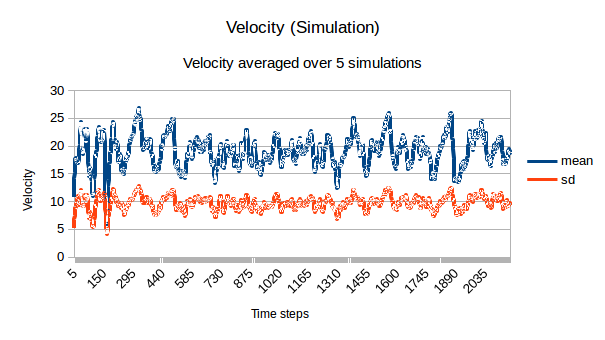
\includegraphics[width=0.8\linewidth]{figs/runs/2svel}
\end{center}
\caption[2. Velocity, robots]{Results from 5 runs averaged on scenario 2, simulator}
\label{fig:res2svel}
\end{figure}
Both of the velocity graphs in the second scenario are considerably lower than the ones found in the other two scenarios. This is expected because one of the four entity is stationary, i.e. non-moving. 
\clearpage
\subsection{Results from scenario 3}
\label{sec:res3}
\begin{figure}[h]
\begin{center}
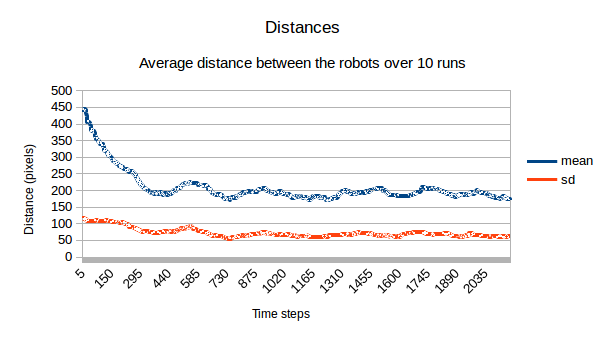
\includegraphics[width=0.8\linewidth]{figs/runs/3pdist}
\end{center}
\caption[3. Distances, robots]{Results from 10 runs averaged on scenario 3, robots}
\label{fig:res3pdist}
\end{figure}
\begin{figure}[h]
\begin{center}
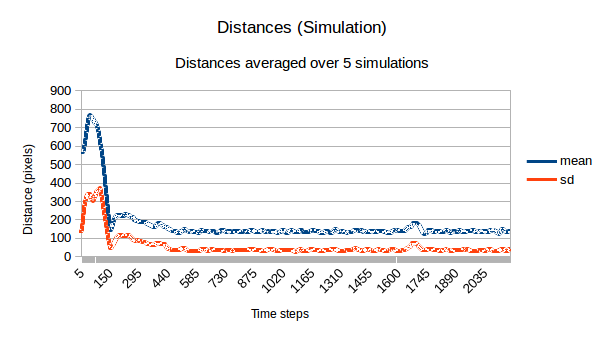
\includegraphics[width=0.8\linewidth]{figs/runs/3sdist}
\end{center}
\caption[3. Distances, simulation]{Results from 5 runs averaged on scenario 3, simulator}
\label{fig:res3sdist}
\end{figure}
The third scenario consists of entities that are placed randomly, the purpose behind this is to check that flocking and collision avoidance are still intact. Both the first and the second scenario were designed to check a specific behavior, this third scenario is not testing any specific behavior.

The results for the distances between the robots in the third scenario is similar to the one in the first. They move closer to each other, and then stay as a flock for the rest of the time. In the simulator, the Boids starts by moving further away from each other, before converging together.
The Boids that starts on the lower right are behind an obstacle, which pushes it away from the other ones. The lower left Boid has a start velocity away from the robots, and due to the short cohesion distance radius, it will move away from the other Boids. The other Boids are not in range for the cohesion behavior to activate.
However it does not take too long before the Boids are able to flock together, as seen from figure \ref{fig:res3sdist} the robots are starting to move towards each other after 40 time steps, and are fully flocked together at time step 150. 
The robots does not have the same behavior as the Boids in this scenario, and they have a much wider cohesion distance. Obstacles do not push the robots in the opposite direction either, when a robot tries to figure out which direction it is going to move in, it will ignore the wall and obstacles. If there is an obstacle in front of a robot, it will turn away from the obstacle. But the next time it calculates where it wants to go, it might calculate the direction it want to go is through the obstacle, thus the robot will turn toward the obstacle then realize that there is in fact an obstacle in front of it and it has to turn away. The robot might get stuck because of this turning behavior, but it will eventually force itself to move around the obstacle. In the mean time, the other robots will move towards the robot that has been stuck behind the obstacle.

The angle and velocity graph of the third scenario is relatively similar to the graphs in the first scenario.
\begin{figure}[h]
\begin{center}
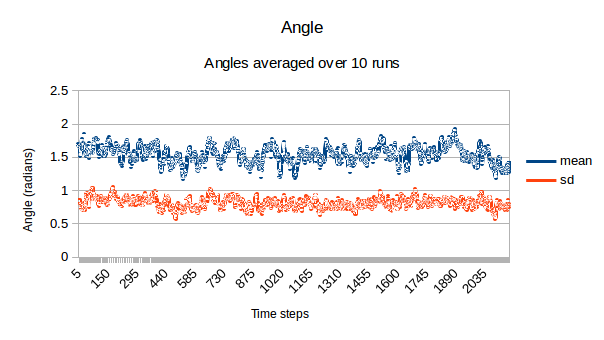
\includegraphics[width=0.8\linewidth]{figs/runs/3pangle}
\end{center}
\caption[3. Angle, robots]{Results from 10 runs averaged on scenario 3, robots}
\label{fig:res3pang}
\end{figure}
\begin{figure}[h]
\begin{center}
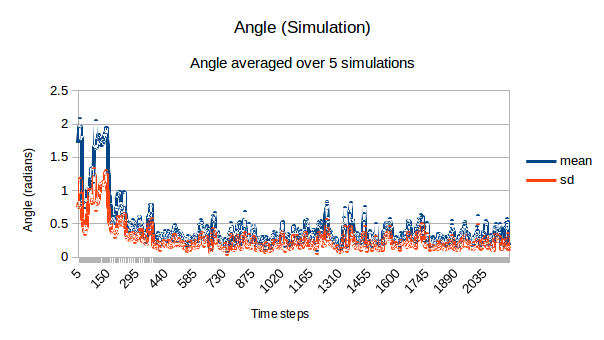
\includegraphics[width=0.8\linewidth]{figs/runs/3sangle}
\end{center}
\caption[3. Angle, robots]{Results from 5 runs averaged on scenario 3, simulator}
\label{fig:res3sang}
\end{figure}
\begin{figure}[h]
\begin{center}
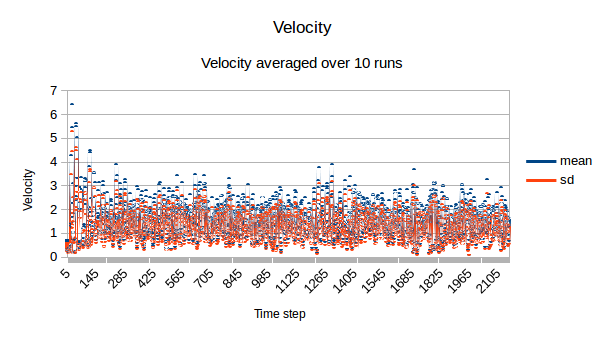
\includegraphics[width=0.8\linewidth]{figs/runs/3pvel}
\end{center}
\caption[3. Velocity, robots]{Results from 10 runs averaged on scenario 3, robots}
\label{fig:res3pvel}
\end{figure}
\begin{figure}[h]
\begin{center}
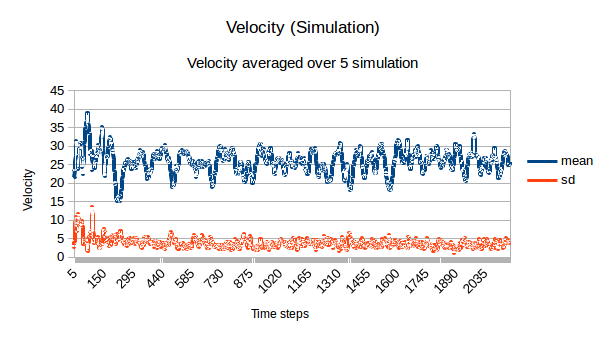
\includegraphics[width=0.8\linewidth]{figs/runs/3svel}
\end{center}
\caption[3. Velocity, robots]{Results from 5 runs averaged on scenario 3, simulator}
\label{fig:res3svel}
\end{figure}

\clearpage
\section{Discussion}
\label{sec:discussion}
This section will mainly focus on explaining the overall data from the results, why there is a difference between the physical experiment and the experiments done in a simulator.

The robots are able to flock faster in the first and third scenario than the robots in the second scenario. This might be because each of the robot start out by themselves and will therefore seek the other ones.
The equilibrium distance which the Boids are flocking at, seems to be around 120 px to 150 px. As mentioned earlier, the separation distance of the Boids is 120 px.
The separation distance for the robot is slightly increased compared to the Boids', the distance is 150 px instead of 120 px. The robots are not only influenced by the separation vector for collision avoidance, but they use their distance sensors as well. So it is expected that the equilibrium distance between the robot is not exactly at 150 px, according to the graphs, the robots' flocking distance stays around 200 px.
%The distances converges to 200 px in about 300-400 time steps for the robots in the first scenario and the third scenario. In the first and third scenario, the robots' distance converges to 200 px, and the simulator converges to 150 px. These numbers comes from the behaviors explained in section \ref{sec:experimentalSetup}. The separation distance is 120 px, so the Boids will try to stay around 120 px away from the other Boids. The same goes for the robot, but due to the distance sensors used for avoiding obstacles, they tend to stay further away from the other robots. 

%In the first and third scenario, each robot starts alone. Due to this, only the sensors used for obstacle avoidance, the "away from wall" and the cohesion behavior will be active. This makes each of the robot move towards the other ones, and the robots converge to a flock faster. 

%//angle
The angles measured seems to vary a lot, even if the alignment behavior tries to make all the robots face the same way. But the overall trend of the robots seems to be that the angles lingers around 1.5 radians on average for all three scenarios, which is pretty high.

The simulated Boids are able to face in the same direction as the other Boids, starting with an angle difference of 2 radians and slowly dropping down to 0.5 radians. This holds true on the graphs shown for the first and third scenario. The angles in second scenario are varying a lot, ranging from 0.4 radians to 1.6. This happens because one of the Boid is not moving, its angle is always 0. While the other three is moving around and their will range from $-\pi$ to $\pi$ depending on the direction they are moving.

If the allowed space to travel were bigger, and there were no obstacles. The Boids would be able to move without needing to turn, and the angle between them would stay consistently low. However the allowed space for the robots to travel is limited and there is an obstacle there as well.
Whenever the robots detects an obstacle or move towards the walls, the distance sensors will make the robot turn around so the robot will not crash. Sometimes the robots will think that the other robots around itself are obstacles as well, because it has no way to tell the difference between the robots from an actual obstacle. This is because the distance sensors can not distinguish anything, it only measures a distance and the robots will try to avoid anything that is too near it, thinking that the object it detects is an obstacle.

The velocity for the robot varies a lot, we can see from the graph that the velocity varies from 0 to 6.3. The watcher software logs the velocity data by finding the change in position between two time steps, that is it finds $\Delta P$ as shown in equation \ref{eq:calcrobvel} of each robot every iteration. When a robot is turning to change direction or to avoid an obstacle, it is not moving because it is just spinning in place. 

The method used to measure the velocity of the robot is very imprecise, when logging the velocity of a robot with constant max velocity, the results did not stay consistently at a given number. 

The result from this test is shown in figure \ref{fig:speed}, the robot is moving at max speed the whole time but there is no consistent line in the graph. The graph consists of "pillars", meaning that the graph goes from 12 to 0 and back up to 12 again. The big gaps in the graph is when the robot has encountered the wall and stops to turn away.

\begin{figure}[h]
\begin{center}
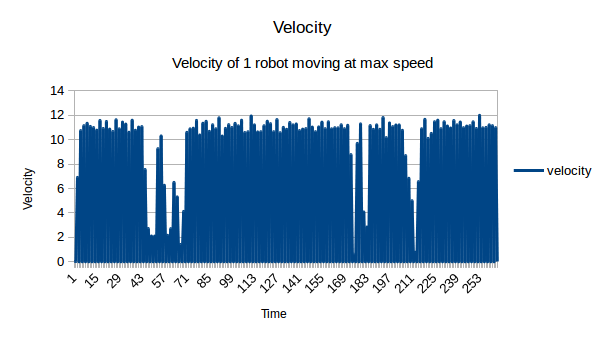
\includegraphics[width=0.8\linewidth]{figs/speed}
\end{center}
\caption[Velocity of robot]{One robot moving at max velocity, only turning when facing a wall}
\label{fig:speed}
\end{figure}

The Boids in the simulator never stops, that is why the velocity never drops down to 0, they keep moving in different direction all the time. Being able to move freely in all 360\textdegree\ almost instantly. They do not need to stop to change direction.
The physical ChIRP robot needs to turn around before moving in a new direction. As long as the new direction is off by an angle larger than 1\textdegree\ from the angle the robot is currently facing, then it will stop and turn. All turning takes approximately one second, before the robot is moving again. If the robot will turn a lot, it will only have one second to do so, before it has to move. If it only needs to turn 2\textdegree, it will turn first and wait until it has been one second before moving on.
The one second delay is introduced to keep the timing somewhat synchronous between the robots, one second delay is long enough for the robot to be able to almost turn all the way around (180\textdegree). 


The graphs only shows the average distance between the robots, the velocity of the robots and the difference between their angle. The graphs do not show where the robots are moving or whether they have crashed into anything.
Sometimes the robots do bump into the obstacles, or the other robots. The reason is that the robots measures the distances before moving, and not continuously while moving. So if a robot measures the distance in front of it and there is no obstacle in front of it, it will start to move forward. When the robot moves forward it might hit an obstacle or robot if the object is too close to it when it measures the distance. Sometimes robots moves onto the path of another robot while the other robot is moving, the other robot will probably bump into the one blocking its path. The robots do  crash into each other sometimes, that is they do push each other around when they are trying to occupy the same space as the other robots. This might happen if both robots are measuring the distances around them, and either some disturbances make the distance measured inaccurate or the other robots move into the other ones' path between the time they are doing the distance measuring.

When the robots bump into each other, they nudge each other and might scrape against the surface of each other. However none of the paper taped on the robot has been torn apart when the robots were scraping against each other while running the experiment.

The robots only moves forward, and they only turn when they need to change direction or if there is an object in front of it that it needs to avoid. Sometimes the robots suddenly stops and rotates on the spot as if there is some sort of object in front of it, even if there is none.
Whenever the robot turns, the watcher will not see any change in position, which is the method it uses to log the velocity of the robots. The watcher will therefore log that the velocity of the robot is 0 when the robots turn around on the same spot. 
The distance measured by the robot's sensors might be imprecise, due to disturbances around in the room that makes the measured distances imprecise. The disturbances can come from the infrared light the other robots sends out when they are measuring distances themselves, which might bounce around in the sandbox and disturb the other robots. 

For the camera to see the two colored post it notes on the robots, the room needs to be well lit. Extra lights were placed around the sandbox to lit it up. The room where the experiment took place had two large windows, by daytime the sun would shine into the room. The sunlight contains infrared light, if the sun shines into the room and hits the area where the robots roam, the robot will sense the infrared lights from the sunshine and think that there is an object in front of it. The blinds in the room were closed, but some of the sun would always shine into the room.




\chapter{Evaluation and Conclusion}
\label{cha:evaluationAndConclusion}

%{\it Lorem ipsum dolor sit amet, consectetur adipiscing elit. Nam consequat pulvinar hendrerit. Praesent sit amet elementum ipsum. Praesent id suscipit est. Maecenas gravida pretium magna non interdum. Donec augue felis, rhoncus quis laoreet sed, gravida nec nisi. Fusce iaculis fermentum elit in suscipit. }

\section{Evaluation}
\label{sec:Evaluation}

%When evaluating your results, avoid drawing grand conclusions, beyond that which your results can in fact support. Further, although you may have designed your experiments to answer certain questions, the results may raise other questions in the eyes of the reader. It is important that you study the graphs/tables to look for unusual features/entries and discuss these aswell as discussing the main findings in the results. 




\section{Contributions}~\label{cont}
\label{sec:Contributions}

%What are the main contributions made to the field and how significant are these contribution.  

\section{Future Work}
\label{sec:futureWork}

%TODO write intro to this chapter here
This section will look further upon what research question is still unanswered and what can be improved.

\textbf{More robots}
The current implementation of the system only supports four simultaneous robots at the same time. A new robot can not be added to the system without uploading the code to each robot in use, nor can a robot disappear from the system. The camera tracking software loads a configuration file at startup that specifies how many robots will be tracked, this value has to be manually changed by the user and reloaded.
The watcher software needs to know which robot on its screen belongs to which bluetooth serial port. If one of the robots' bluetooth connection disconnects or times out, everything has to stop and reconnected again for it to work.

The main idea behind swarm robots is that it should be able to run continuously without having to reboot or stop the swarm to add a new robot or remove one. If one of the entity in a swarm is defected, injured or not working, the other ones should still be operable.

The current implementation of this project relies on the robot needing to know how many other robots there will be in the sandbox at the same time, because it will need to know how much data it is going to store before processing it. This has to be changed manually in the code and then uploaded to the robot again.
A working flocking flock should have more than four robots running simultaneously, and we should be able to add a new robot without re-uploading the code to the robots.

\textbf{More fluid movement} %TODO rewrite
The current implementation does not punish the robot for standing still nor for only rotating on the same spot. The only escape from continuously spinning on the same spot is a spin counter, which forces the robot to move forward if the robot has been stuck on a spot for five iterations and if there is nothing in front of it. 

Each robot also stops when it turns around and whenever they need to change direction. When birds fly together as a flock they do not stop when they need to turn. The robots should be able to move and rotate without stopping.

%In scenario 2, the robots do move around the obstacle, but this does not happen at the same time. 

%[From template] %TODO remove
%Consider where you would like to extend this work. These extensions might either be continuing the ongoing direction or taking a side direction that became obvious during the work. Further, possible solutions to limitations in the work conducted, highlighted in ~\ref{sec:Discussion} may be presented. 





\backmatter

\addcontentsline{toc}{chapter}{Bibliography}
\bibliography{citations}
\nocite{*}
\let\cleardoublepage\clearpage
\appendix
\label{cha:appendices}
\chapter{Camera tracking configuration file}
\label{app:opencvcfg}
chirpObserverConfig.cfg
\begin{lstlisting}
# [comPort]
# the id of the comm port to use. 
# 0 corresponds to /dev/ttyS0 
# 1 corresponds to /dev/ttyS1
# 2 corresponds to /dev/ttyS2
# 3 corresponds to /dev/ttyS3
# 4 corresponds to /dev/ttyS4
# 5 corresponds to /dev/ttyS5
# 6 corresponds to /dev/ttyS6
# 7 corresponds to /dev/ttyS7
# 8 corresponds to /dev/ttyS8
# 9 corresponds to /dev/ttyS9
# 10 corresponds to /dev/ttyS10
# 11 corresponds to /dev/ttyS11
# 12 corresponds to /dev/ttyS12
# 13 corresponds to /dev/ttyS13
# 14 corresponds to /dev/ttyS14
# 15 corresponds to /dev/ttyS15
# 16 corresponds to /dev/ttyUSB0
# 17 corresponds to /dev/ttyUSB1
# 18 corresponds to /dev/ttyUSB2
# 19 corresponds to /dev/ttyUSB3
# 20 corresponds to /dev/ttyUSB4
# 21 corresponds to /dev/ttyUSB5
# 22 corresponds to /dev/ttyAMA0
# 23 corresponds to /dev/ttyAMA1
# 24 corresponds to /dev/ttyACM0
# 25 corresponds to /dev/ttyACM1
# 26 corresponds to /dev/rfcomm0
# 27 corresponds to /dev/rfcomm1
# 28 corresponds to /dev/ircomm0
# 29 corresponds to /dev/ircomm1
# id = 27

[camera]
# the id of the camera device to use, numbered from 0 and upwards
# deviceId = 1
deviceId = 0
# the width and height of the captured image, denoted in pixels
width = 720	
height = 500
# the maximum number of objects to track. 
#All objects are ignored if the number of objects
# discovered exceeds this number
maxNumObjects = 1000
#the minimum object area to recognize (in pixels). 
#Any object smaller than this is ignored.
minObjectArea = 10
# upper limit of the size of leds compared to 
# min(frame width, frame height)
ledSize = 0.01

# settings governing the colors in the captured frame
# the settings are potentially specific to each camera
# linux application "guvcview" provides details
# the settings appear to be sticky, so an application like 
#"guvcview" may be necessary to revert to default state
#
# if the value is less than 0, the application won't change
# the camera's setting for that property
# the brigtness of the image
brightness = 0.1
# the contrast of the image (0 - 10 with default of 5)
contrast = 5
# the saturation of the image (0 - 200 with default of 83)
saturation = 30

# each color is defined by six boundries,
#and is only recognized if the HSV value is within the bounds
[red]
hmin = 120
hmax = 220
smin = 100
smax = 256
vmin = 130
vmax = 256

#hmin = 0
#hmax = 45
#smin= 90
#smax = 256
#vmin = 170
#vmax = 256

[blue]
hmin = 100
hmax = 120
smin = 250
smax = 256
vmin = 250
vmax = 256

[green]
hmin = 31
hmax = 90
smin = 100
smax = 256
vmin = 135
vmax = 256

#hmin = 21
#hmax = 86
#smin= 50
#smax = 256
#vmin = 205
#vmax = 256

# the size of the virtual feed depicting the 
#scene as interpreted by the tracker
[virtualFeed]
width = 500
height = 500
 
# settings for the UDP network sending 
#information about tracked robots
[network]
enabled = true 
address = localhost
port = 52346

[general]
# whether to calibrate colors, this allows one to 
#find values for the color definitions
calibrationEnabled = false
# the time the system waits after a frame 
#has been processed before it fetches a new one
# if this number is set too low, 
#the camera won't be able to finish capturing a frame
frameDelay = 10

[tracking]
# number of robots to track
numRobots = 4
# robots are removed if this number of steps pass 
#without a pinpointing of the robot's position
evictionLimit = 6
# the maximum speed (distance / frame) of robots in any 
#direction compared to the width and height of the bounding box
 robotSpeed = 0.01
# robotSpeed = 0.065
# the maximum rotational speed (radians / frame) of
# the robot compared to a full circle
robotRotationalSpeed = 0.05
# the diameter of the robots compared to the bounding box
robotDiameter = 0.06
#0.059
# the number of recent values to use when smoothing
# the position and rotation of the robot
historyLength = 3

[controls]
# key to reload the configuration at run time. 
#Not all changes will take effect
loadConfig = l
\end{lstlisting}
\chapter{Sorting algorithms}
\label{app:sorting} This section will explain some of the sorting algorithms that are used in some of the papers mentioned in chapter \ref{sec:background}. 
\section{Odd even sort}
Odd even sort is a sorting algorithm which resembles bubble sort. The algorithm takes a list of elements, then compares all the odd placed element with the element next to it. That is; compare list[i] with list[i+1] where $i$ is an odd number. Then the algorithm does the same for all $i$ even number. This is done repeatedly until we get a sorted list.

\section{Bitonic sort}
Bitonic sort is a highly parallel sorting algorithm, the idea is to have the elements in the list in a bitonic sequence. A bitonic sequence is a sequence where the list is increasing, then decreasing and then eventually increasing again. However the last increasing part are not allowed to increase past the first element in the list.
\begin{figure}[H]
    \centering
    \includegraphics[width=0.8\linewidth]{images/bitonicseq}
    \caption[Sequence of elements]{Left figure is a bitonic sequence, right figure is not a bitonic sequence because the last increasing part is higher than the start}\label{fig:bitonicseq}
\end{figure}
After the algorithm have obtained a bitonic sequence, it will start to compare the elements with certain distance from each other and swap these elements if they are in the wrong order.
\begin{figure}[H]
    \centering
    \includegraphics[width=0.8\linewidth]{images/bitonicexample}
    \caption{Example of a bitonic sort run}\label{fig:bitonicex}
\end{figure}
In the example we have the numbers 11,13,14,37,16,7,4,1. Which is initially in a bitonic sequence because the first half is increasing and the last half is decreasing. The algorithm now compares the first and the fifth element, as indicated by the arrows. All of these comparisons can be done in parallel. The algorithm compares the elements at different position, in the example it start with a comparison of elements that are distance 4 away from each other, that is element at position 1 and 5, 2 and 6 and so on. Then elements with distance 2 is compared, and then elements with distance 1 are compared.
The runtime of the bitonic sort algorithm is $O(nlog(n)^2)$ but the idea is to run it on $n$ Cuda threads, reducing the runtime to $O(log(n)^2)$ for each thread.


\end{document}
